% ============================================================
% www-paper-springer.tex
% Target: World Wide Web: Internet and Web Information Systems (Springer)
% Format: Springer Nature journal formatting guidelines
% Note: Uses article class for compilation compatibility.
%       For final submission, the production team reformats
%       using sn-jnl.cls after acceptance (per journal policy).
% Reference style: Numbered [n] with sn-basic.bst
% ============================================================

\documentclass[11pt,a4paper]{article}

\usepackage[T1]{fontenc}
\usepackage[utf8]{inputenc}
\usepackage{lmodern}
\usepackage[margin=25mm]{geometry}
\usepackage{pgfplots}
\pgfplotsset{compat=1.18}
\usepackage{tikz}
\usetikzlibrary{shapes.geometric, arrows.meta, positioning, calc, decorations.pathreplacing, patterns, fit}
\usepackage{booktabs}
\usepackage{array}
\usepackage{graphicx}
\usepackage{float}
\usepackage{enumitem}
\usepackage{amsmath}
\usepackage{amssymb}
\usepackage{amsthm}
\usepackage{listings}
\usepackage{multirow}
\usepackage{tabularx}
\usepackage{algorithm}
\usepackage{algorithmic}
\usepackage{pifont}
\usepackage{subcaption}
\usepackage{xcolor}
\usepackage[numbers,sort&compress]{natbib}
\usepackage{hyperref}

% Springer bst compatibility
\providecommand{\bibcommenthead}{}
\providecommand{\bibinfo}[2]{#2}

\hypersetup{
    colorlinks=true,
    linkcolor=springerblue,
    urlcolor=springerblue,
    citecolor=springerblue
}

\setlength{\emergencystretch}{3em}

\theoremstyle{plain}
\newtheorem{theorem}{Theorem}
\newtheorem{proposition}[theorem]{Proposition}
\newtheorem{lemma}[theorem]{Lemma}
\newtheorem{corollary}[theorem]{Corollary}
\theoremstyle{definition}
\newtheorem{definition}[theorem]{Definition}
\theoremstyle{remark}
\newtheorem{remark}[theorem]{Remark}

% Colors
\definecolor{springerblue}{HTML}{1A5276}
\definecolor{accent}{HTML}{C0392B}
\definecolor{chartblue}{HTML}{2874A6}
\definecolor{chartgreen}{HTML}{1E8449}
\definecolor{chartorange}{HTML}{CA6F1E}
\definecolor{chartred}{HTML}{C0392B}
\definecolor{chartpurple}{HTML}{6C3483}
\definecolor{chartgray}{HTML}{5D6D7E}
\definecolor{chartteal}{HTML}{148F77}
\definecolor{codebg}{HTML}{F5F5F5}

\lstset{
    basicstyle=\ttfamily\small,
    backgroundcolor=\color{codebg},
    frame=single,
    framerule=0.4pt,
    rulecolor=\color{gray!40},
    breaklines=true,
    columns=fullflexible,
    keepspaces=true,
    showstringspaces=false,
    tabsize=2,
    xleftmargin=4pt,
    xrightmargin=4pt,
    aboveskip=6pt,
    belowskip=6pt,
    numbers=left,
    numberstyle=\tiny\color{gray},
    numbersep=5pt,
    keywordstyle=\color{springerblue}\bfseries,
    stringstyle=\color{chartgreen},
    commentstyle=\color{chartgray}\itshape,
    language=Java,
}

% ============================================================
\begin{document}
% ============================================================

\title{Constrained Self-Service Group Formation on Serverless\\ NoSQL Infrastructure: A Deployed Reference Architecture\\ and Experience Report}

\author{
Mithun Gowda B\textsuperscript{a}, Harsha N\textsuperscript{a}, Naren V\textsuperscript{a}, Nevil Anson Dsouza\textsuperscript{a}\\
NV Sushma\textsuperscript{b}, A S Manjunatha\textsuperscript{b}\textsuperscript{*} \\[4pt]
\small \textsuperscript{a}Department of Computer Science and Engineering,\\
\small Don Bosco Institute of Technology (Affiliated to VTU), Kumbalagodu, Bangalore 560074, India\\
\small \textsuperscript{b}Department of Chemistry,\\
\small Don Bosco Institute of Technology (Affiliated to VTU), Kumbalagodu, Bangalore 560074, India\\[2pt]
\small \textsuperscript{*}Guide and corresponding author email: \texttt{madhumanjuas@dbit.co.in}
}
\date{}

\maketitle

\begin{abstract}
Self-service web platforms that let end users form their own groups under composition rules must enforce those rules at the moment of user action, maintain cross-document invariants on document-store infrastructure, and operate inside the quotas of third-party services. This paper is an experience report on a reference architecture for that problem, deployed in production for an engineering cohort with an enrolment roster of 823 students and released as open source.

We contribute three things. First, a parameterised composition model whose mandatory-representation constraint is \emph{disjunctive}, matching the rule the deployment actually enforced, together with a feasibility theorem reduced to three independent conditions. In establishing it we correct an error in our earlier formulation, which asserted a condition that is not in fact necessary, and we note that the general case with overlapping requirement groups is a minimum hitting set problem and therefore not checkable in polynomial time. Second, a two-phase validation design that separates recoverable warnings from irrecoverable blocks during iterative group building, with its complexity and, more importantly, the precise scope of its correctness guarantee stated explicitly. Third, a candid account of what this architecture got wrong. We avoided multi-document transactions although the underlying database provides them, and we placed rate-limiting and quota-spreading state in per-instance memory on a serverless platform where such state does not survive instance recycling. A successor deployment by the same authors reverted the first of these decisions.

We also withdraw a technique reported in an earlier version of this work, which spread outbound email across several free-tier accounts to multiply an effective daily quota. Multiplying a per-account quota in that manner conflicts with the intent of the provider's terms, and we set out the sanctioned alternatives instead. Finally, we retract the previously reported figure of 100\% constraint satisfaction for completed groups: because group completion is gated by the very predicate being measured, that figure is true by construction and carries no information. We state which quantities the deployment genuinely instrumented and which it did not, so that the gap is visible rather than concealed. The implementation comprises 10,937 lines of TypeScript across 58 files and is archived at a fixed commit.
\end{abstract}

\medskip
\noindent\textbf{Keywords:} Self-service web platforms; Group composition constraints; NoSQL data integrity; Serverless architecture; Experience report; Negative results

% ============================================================
\section{Introduction}
\label{sec:introduction}
% ============================================================

\subsection{Problem Statement}

Modern web platforms increasingly adopt self-service models in which end users, rather than administrators, perform complex, multi-step workflows such as group formation, resource allocation, and collaborative project setup. These workflows impose \emph{configurable constraints}: rules that govern the composition of user-formed groups, the distribution of attributes across members, and the conditions under which a group reaches a valid terminal state. Examples include hackathon team composition rules (``at least one designer and one backend developer''), organizational unit staffing policies (``no more than four members from any single department''), and marketplace listing requirements (``minimum two product categories represented'').

Enforcing such constraints in real time, providing immediate feedback as each member is added to an evolving group, is substantially more challenging than batch validation after group formation is complete. The system must evaluate constraint feasibility at every intermediate state, distinguish between violations that can self-correct through subsequent additions (soft warnings) and violations that are irrecoverable (hard blocks), and handle concurrent modifications from multiple users operating on the same group simultaneously.

These challenges are compounded on \textbf{NoSQL document-store infrastructure}, which trades the ACID transaction guarantees of relational databases for horizontal scalability and real-time subscription capabilities~\cite{cattell2010, vogels2009, han2011}. Without multi-document transactions, enforcing cross-document invariants, such as ``each user belongs to at most one group'', requires architectural patterns that are absent from conventional web application frameworks.

A third, often-overlooked challenge arises from \textbf{third-party API rate limits}. Self-service platforms that integrate external services (email delivery, SMS verification, payment processing) must operate within per-key quotas imposed by service providers. During peak usage, such as a registration burst where hundreds of users authenticate within hours, a single API key's daily quota can be exhausted rapidly, causing service degradation precisely when demand is highest.

\subsection{Research Gap}

Existing web systems address these challenges in isolation but not in combination:

\begin{itemize}[noitemsep,topsep=4pt]
    \item \textbf{Real-time web architectures}~\cite{pimentel2012, lubbers2010} enable push-based data delivery via WebSocket~\cite{wang2013} and Server-Sent Events (SSE) but do not address constraint enforcement or data integrity.
    \item \textbf{Constraint satisfaction systems}~\cite{rossi2006, kumar1992} provide formal frameworks for constraint modeling but operate in batch mode, not as real-time web services with concurrent user interactions.
    \item \textbf{NoSQL consistency models}~\cite{brewer2000, gilbert2002, decandia2007} characterize trade-offs between consistency, availability, and partition tolerance but do not prescribe application-level patterns for enforcing multi-document invariants.
    \item \textbf{Serverless computing platforms}~\cite{jonas2017, baldini2017, schleier-smith2021} provide auto-scaling infrastructure but introduce challenges for stateful operations (rate limiting, session management) due to ephemeral function instances.
    \item \textbf{Self-service web platforms}~\cite{bafoutsou2002, olson2000} enable user-driven collaboration but typically lack formal constraint models and comprehensive data integrity guarantees.
\end{itemize}

Each of these strands is mature in isolation. What we did not find, when building the system described here, was a published account of how they compose in a single deployed platform that must answer to real users under a real deadline. That is the gap this paper addresses, and we are careful about its nature: it is a gap in reported engineering experience, not a gap in available techniques. Every mechanism we use is individually known. Fig.~\ref{fig:gap} sketches the region of the design space our deployment occupies; we stress that the axes are qualitative and that the placement of other approaches reflects their design intent as documented by their authors, not measurements we performed.

\begin{figure}[htbp]
\centering
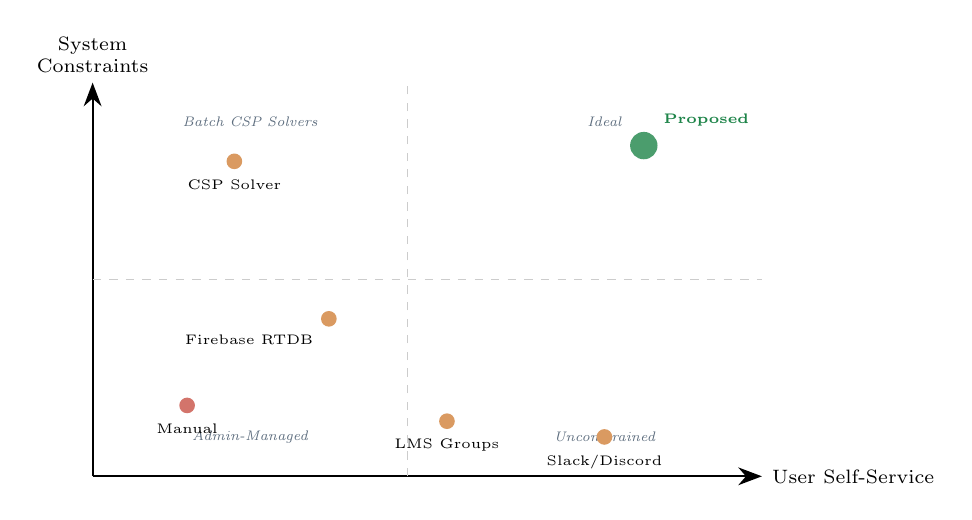
\begin{tikzpicture}[
    every node/.style={font=\small},
    box/.style={draw, rounded corners=4pt, minimum width=2cm, minimum height=1cm, align=center, line width=0.6pt}
]
    % Axes
    \draw[-{Stealth[length=3mm]}, thick] (0,0) -- (8.5,0) node[right, font=\scriptsize] {User Self-Service};
    \draw[-{Stealth[length=3mm]}, thick] (0,0) -- (0,5.0) node[above, font=\scriptsize, align=center] {System\\Constraints};

    % Quadrant labels
    \node[font=\tiny\itshape, color=chartgray] at (2.0, 4.5) {Batch CSP Solvers};
    \node[font=\tiny\itshape, color=chartgray] at (6.5, 4.5) {Ideal};
    \node[font=\tiny\itshape, color=chartgray] at (2.0, 0.5) {Admin-Managed};
    \node[font=\tiny\itshape, color=chartgray] at (6.5, 0.5) {Unconstrained};

    % Existing solutions
    \node[circle, fill=chartred!70, inner sep=2pt, label={[font=\tiny]below:Manual}] at (1.2, 0.9) {};
    \node[circle, fill=chartorange!70, inner sep=2pt, label={[font=\tiny]below:CSP Solver}] at (1.8, 4.0) {};
    \node[circle, fill=chartorange!70, inner sep=2pt, label={[font=\tiny]below:LMS Groups}] at (4.5, 0.7) {};
    \node[circle, fill=chartorange!70, inner sep=2pt, label={[font=\tiny]below:Slack/Discord}] at (6.5, 0.5) {};
    \node[circle, fill=chartorange!70, inner sep=2pt, label={[font=\tiny]below left:Firebase RTDB}] at (3.0, 2.0) {};

    % Our solution
    \node[circle, fill=chartgreen!80, inner sep=3.5pt, label={[font=\tiny\bfseries, color=chartgreen]above right:Proposed}] at (7.0, 4.2) {};

    % Dashed lines for quadrants
    \draw[dashed, gray!40] (4.0, 0) -- (4.0, 5.0);
    \draw[dashed, gray!40] (0, 2.5) -- (8.5, 2.5);
\end{tikzpicture}
\caption{Positioning of web group-formation approaches along user self-service and system constraint enforcement dimensions. Existing solutions cluster in three quadrants; the upper-right quadrant (high self-service + high constraint enforcement) remains unoccupied.}
\label{fig:gap}
\end{figure}

\subsection{Scope and Contributions}

This is an experience report. We make no claim that the individual mechanisms described here are new, and we have removed such claims from an earlier version of this work. Its value, if it has any, lies in the fact that the system was built, deployed, used, and is available for inspection, and that we are willing to describe its defects as precisely as its merits.

\begin{enumerate}[noitemsep,topsep=4pt]
    \item A \textbf{composition model and feasibility result} (Section~\ref{sec:constraints}). The model admits disjunctive mandatory-representation requirements, which is what the deployment actually enforced and what our earlier conjunctive formulation failed to capture. We reduce feasibility to three independent conditions, correct a non-necessary condition asserted in our earlier formulation, and identify the boundary beyond which feasibility checking becomes NP-hard.

    \item A \textbf{two-phase validation design and its honest correctness scope} (Section~\ref{sec:constraints}). We state what the two phases do and do not guarantee. In particular we make explicit that the guarantee is conditional on serialised application of the validator, which the original deployment did not ensure.

    \item An \textbf{account of three design decisions we now consider mistaken} (Sections~\ref{sec:integrity}, \ref{sec:security}, and~\ref{sec:discussion}): avoiding multi-document transactions that the database provides, holding rate-limiter state in per-instance memory on a serverless runtime, and spreading email across multiple free-tier accounts. For each we give the reasoning at the time, the consequence, and what we would do instead.
\end{enumerate}

\noindent\textbf{What this paper does not claim.} It does not claim a novel constraint-satisfaction algorithm; the validator is a linear scan over a small member list. It does not claim generality beyond its single deployment. It does not claim measured superiority over the alternative approaches discussed in Section~\ref{sec:evaluation}, and we have removed the scored comparison that appeared in an earlier version because we had no methodology capable of supporting it.

The remainder of this paper is organized as follows. Section~\ref{sec:related} surveys related work across seven research areas. Section~\ref{sec:model} presents the system model and design principles. Section~\ref{sec:constraints} formalizes the constraint model with feasibility and correctness proofs. Section~\ref{sec:architecture} describes the system architecture, including the round-robin API key rotation. Section~\ref{sec:integrity} details the six-layer data integrity framework. Section~\ref{sec:security} presents the security architecture. Section~\ref{sec:evaluation} reports the production evaluation results. Section~\ref{sec:discussion} discusses findings and limitations. Section~\ref{sec:future} outlines future work. Section~\ref{sec:conclusion} concludes.

% ============================================================
\section{Related Work}
\label{sec:related}
% ============================================================

\subsection{Real-Time Web Architectures}

The evolution from polling-based to push-based web architectures has enabled a new class of interactive applications. The WebSocket protocol~\cite{pimentel2012} provides full-duplex communication over a single TCP connection, enabling server-initiated data delivery without the overhead of HTTP long-polling. Lubbers and Greco~\cite{lubbers2010} demonstrate that WebSocket reduces latency by 3:1 and bandwidth by 500:1 compared to HTTP polling for high-frequency data streams. Server-Sent Events (SSE)~\cite{grigorik2013} provide a simpler, unidirectional alternative suitable for scenarios where the server pushes updates to clients without requiring bidirectional communication.

Firebase Firestore~\cite{firebase} implements a document-level subscription model through its \texttt{onSnapshot} API, which pushes data changes to connected clients whenever the subscribed document is modified. Unlike WebSocket-based architectures that require explicit server-side event emission, Firestore's subscription model is declarative: clients subscribe to document paths, and the infrastructure handles change detection, conflict resolution, and delivery. This model is particularly well-suited for applications where multiple users observe shared state (e.g., group composition) and require immediate visual feedback when that state changes.

However, real-time delivery infrastructure alone does not address the \emph{semantic} challenge of constraint enforcement. Existing real-time web frameworks provide the communication substrate but leave application-level invariants, such as group composition rules, membership uniqueness, and state-machine transition validity, entirely to the application developer. Our work builds on Firestore's real-time capabilities while adding a formal constraint layer and multi-level integrity guarantees.

\subsection{Automated and Self-Service Group Formation}

Group formation has an established literature, and it is important to be clear about where our model sits within it. Lappas et al.~\cite{lappas2009} formalise team formation over a social network and establish its NP-hardness; Anagnostopoulos et al.~\cite{anagnostopoulos2012} extend this to an online setting in which tasks arrive over time. Both treat formation as an \emph{optimisation} problem solved \emph{on behalf of} the participants. Sun et al.~\cite{sun2026} report a deployed two-phase procedure for an engineering cohort of 238 students, combining graph clustering with simulated annealing under balance and isolation penalties, and release verification artefacts.

Our problem is deliberately weaker, and this is the honest answer to the question of what differentiates it. We do not optimise an objective and we do not assign anyone to a group. Users choose, and the system's only job is to decide, in constant time and at the instant of a click, whether a proposed addition can still lead to a valid group. Consequently our feasibility result is not a competitor to the optimisation results above: it is a much simpler admissibility question, and we claim only that stating it precisely is useful for implementers, not that it is deep. Where prior work asks which partition is best, we ask which single addition is permissible. We are not aware of a prior statement of necessary and sufficient parameter conditions for this admissibility question in the disjunctive-requirement form of Section~\ref{sec:constraints}, but we regard the result as elementary and would not be surprised to find it as folklore.

\subsection{Constraint Satisfaction in Web Systems}

Lappas et al.~\cite{lappas2009} formalize team formation as a constrained optimization problem on social networks and establish its NP-hardness for the general case where both team quality and inter-member communication cost must be optimized simultaneously. Their approximation algorithms provide provable guarantees for offline settings where all candidates are known in advance.

Anagnostopoulos et al.~\cite{anagnostopoulos2012} extend this to \emph{online} settings where members arrive sequentially and assignments are irrevocable, a model closer to self-service web platforms where users register and join groups over extended periods. Their competitive analysis shows that online algorithms achieve ratios within constant factors of offline optima for practical constraint structures.

Wi et al.~\cite{wi2009} apply genetic algorithms to optimize team competency coverage, demonstrating that evolutionary approaches handle complex multi-objective constraints in R\&D settings.

The constraint satisfaction programming (CSP) literature~\cite{rossi2006, kumar1992, tsang1999} provides the formal foundations for constraint modeling, including arc consistency, backtracking search, and constraint propagation. However, CSP solvers operate in batch mode, they compute complete solutions after all variables and constraints are specified, and are not designed for the interactive, incremental constraint evaluation required by real-time web platforms. Our constraint model draws on CSP formalism (parameterized rules, feasibility analysis) while adapting the evaluation strategy for real-time, per-operation validation.

\subsection{NoSQL Data Integrity}

Brewer's CAP theorem~\cite{brewer2000}, formalized by Gilbert and Lynch~\cite{gilbert2002}, establishes that distributed systems cannot simultaneously guarantee consistency, availability, and partition tolerance. NoSQL databases such as Amazon DynamoDB~\cite{decandia2007} and Google Cloud Firestore~\cite{firebase} prioritize availability and partition tolerance, offering eventual consistency~\cite{vogels2009} or strong consistency within bounded scopes (e.g., single-document reads in Firestore).

The absence of multi-document ACID transactions in many NoSQL systems creates a fundamental challenge for web applications that must enforce cross-document invariants. Cattell~\cite{cattell2010} surveys NoSQL data stores and identifies the lack of referential integrity enforcement as a key trade-off. Stonebraker~\cite{stonebraker2010} argues that this trade-off is acceptable for workloads that are partitionable by entity, but problematic for workloads requiring cross-entity consistency.

Chang et al.~\cite{chang2006} describe Bigtable's single-row transaction model, which provides atomicity for operations within a single entity but not across entities. Firestore extends this with single-document atomicity and limited multi-document transactions (up to 500 documents per batch), but cross-collection invariants still require application-level enforcement.

Our six-layer data integrity framework (Section~\ref{sec:integrity}) addresses this gap by implementing invariant enforcement at multiple application levels, UI guards, API-layer validation, and database security rules, providing defense-in-depth integrity without relying on database-level transactions.

\subsection{Serverless Architecture Patterns}

Jonas et al.~\cite{jonas2017} introduce the serverless computing paradigm, arguing that auto-scaling, pay-per-use cloud functions democratize access to scalable infrastructure. The Berkeley view on serverless computing~\cite{jonas2019} identifies key challenges: cold-start latency, limited execution duration, and the absence of persistent local state.

Baldini et al.~\cite{baldini2017} survey serverless computing patterns and identify stateful serverless applications as an open problem. McGrath and Brenner~\cite{mcgrath2017} benchmark serverless function performance across providers, finding that cold-start latencies range from 100ms to several seconds depending on runtime and provider.

Schleier-Smith et al.~\cite{schleier-smith2021} argue that the next phase of serverless computing must address state management, proposing programming models that integrate state into the serverless paradigm.

Our architecture operates within the constraints of current serverless platforms: in-memory state (rate-limit counters) is tolerated as best-effort and resets on cold starts; persistent state resides entirely in the NoSQL database; and API key rotation is stateless modulo a single in-memory counter. This design achieves zero-cost deployment on free tiers while accepting the trade-offs inherent in serverless infrastructure.

\subsection{Rate Limiting and API Key Management}

Rate limiting is a foundational mechanism for protecting web services from abuse and ensuring fair resource allocation. The token bucket and leaky bucket algorithms~\cite{tanenbaum2011} are widely deployed in API gateways and reverse proxies. The IETF has proposed standardized rate-limit response headers~\cite{ietf-ratelimit2024} to communicate quota status to clients.

Raghavan et al.~\cite{raghavan2007} address distributed rate limiting in cloud environments, proposing algorithms that maintain global rate limits across geographically distributed enforcement points. Their work focuses on \emph{incoming} request rate limiting (protecting the server), whereas our round-robin algorithm addresses \emph{outgoing} request rate limiting (operating within external API quotas), a complementary but distinct problem.

The specific challenge of multiplying effective API capacity through multi-key rotation has received little formal treatment in the literature. Commercial platforms (SendGrid, Brevo, Mailgun) document per-key quotas but do not provide client-side rotation algorithms. Our round-robin approach (Section~\ref{subsec:roundrobin}) formalizes this pattern with complexity analysis and fault-tolerance properties.

\subsection{Self-Service Platforms and Workflow Management}

Self-service web platforms enable end users to perform workflows previously requiring administrator intervention. Van der Aalst et al.~\cite{vanderaalst2003} survey business process management systems, identifying workflow patterns that recur across domains. Harel's statecharts~\cite{harel1987} provide a visual formalism for modeling complex system behavior, including concurrent states and hierarchical decomposition.

Finite state machines (FSMs) are widely used to model entity lifecycle in web applications~\cite{hopcroft1971}. Our system employs FSMs for two critical state transitions: group status (forming $\rightarrow$ full $\rightarrow$ locked) and invitation status (pending $\rightarrow$ approved/rejected/expired). The FSM model ensures that terminal states are immutable and that concurrent transition attempts are handled idempotently.

Bafoutsou and Mentzas~\cite{bafoutsou2002} classify collaborative systems by functionality, identifying group formation, awareness, and communication as core capabilities. Olson and Olson~\cite{olson2000} study distance collaboration, emphasizing the importance of shared awareness of group state, a requirement our real-time subscription architecture directly addresses.

\subsection{Web Application Security}

The OWASP Top Ten~\cite{owasp2021} identifies injection, broken authentication, and cross-site scripting (XSS) as the most critical web application security risks. Barth et al.~\cite{barth2008} provide robust defenses against cross-site request forgery (CSRF), including the \texttt{SameSite} cookie attribute that our implementation employs.

JWT~\cite{jones2015} provides a compact, self-contained token format for session management. Hardt~\cite{hardt2012} defines the OAuth 2.0 framework for delegated authorization. Stuttard and Pinto~\cite{stuttard2011} and Zalewski~\cite{zalewski2012} provide comprehensive treatments of web application attack vectors and of the browser behaviours that defences must account for.

Our five-layer security model (Section~\ref{sec:security}) implements defense-in-depth~\cite{owasp2021} with OTP-based authentication~\cite{mraihi2011}, JWT sessions, database-level access control, transport security headers, and IP-based rate limiting. This architecture is designed for environments where institutional single sign-on (SSO) is unavailable, a common constraint in platforms serving users who lack pre-existing organizational credentials.

% ============================================================
\section{System Model}
\label{sec:model}
% ============================================================

\subsection{Design Principles}

The platform is designed around five principles derived from web systems research:

\begin{enumerate}[noitemsep,topsep=4pt]
    \item \textbf{User self-service:} Users initiate group creation, select members, and choose which groups to join, enabling autonomous workflow completion without administrator intervention.
    \item \textbf{Automated constraint enforcement:} Every member addition is validated against configurable composition rules in real time, preventing invalid group configurations at the point of user action rather than through post-hoc administrative review.
    \item \textbf{Progressive guidance:} Soft warnings guide users toward constraint satisfaction during intermediate group-building stages, with hard blocks only at the point of violation or group completion. This design respects human decision-making processes by providing information at the point when it becomes actionable.
    \item \textbf{Data integrity by design:} Duplication prevention, idempotent operations, and cascade cleanup are built into every state transition, not bolted on after the fact. Invariants are enforced at multiple application levels (defense-in-depth).
    \item \textbf{Platform governance:} Gate controls, bulk data management, real-time statistics, and intervention capabilities provide administrative oversight without micromanagement of individual user workflows.
\end{enumerate}

\subsection{Workflow Model}

The group formation process follows four phases (Fig.~\ref{fig:workflow}):

\begin{figure}[htbp]
\centering
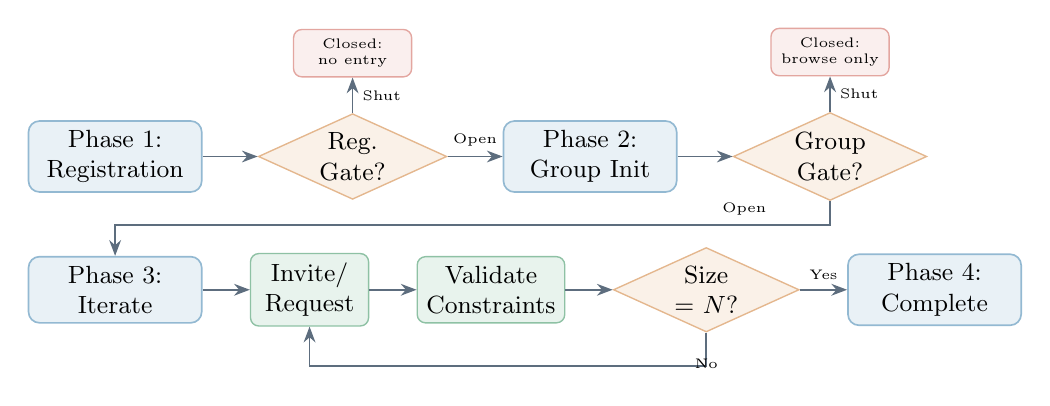
\begin{tikzpicture}[
    node distance=0.5cm and 0.6cm,
    every node/.style={font=\small},
    phase/.style={draw, rounded corners=4pt, minimum width=2.2cm, minimum height=0.8cm, align=center, fill=chartblue!10, draw=chartblue!50, line width=0.6pt},
    gate/.style={draw, diamond, aspect=2.2, minimum width=1.2cm, align=center, fill=chartorange!10, draw=chartorange!50, line width=0.5pt, inner sep=1pt, font=\small},
    act/.style={draw, rounded corners=3pt, minimum width=1.5cm, minimum height=0.6cm, align=center, fill=chartgreen!10, draw=chartgreen!50, line width=0.5pt},
    arrow/.style={-{Stealth[length=2mm]}, draw=chartgray, semithick}
]
    % Phase 1
    \node[phase] (reg) {Phase 1:\\Registration};
    \node[gate, right=0.7cm of reg] (reggate) {Reg.\\Gate?};

    % Phase 2
    \node[phase, right=0.7cm of reggate] (team) {Phase 2:\\Group Init};
    \node[gate, right=0.7cm of team] (teamgate) {Group\\Gate?};

    % Phase 3
    \node[phase, below=0.8cm of reg] (grow) {Phase 3:\\Iterate};
    \node[act, right=0.6cm of grow] (invite) {Invite/\\Request};
    \node[act, right=0.6cm of invite] (validate) {Validate\\Constraints};
    \node[gate, right=0.6cm of validate] (full) {Size\\= $N$?};

    % Phase 4
    \node[phase, right=0.6cm of full] (done) {Phase 4:\\Complete};

    % Negative outcomes of the two administrative gates
    \node[act, above=0.45cm of reggate, fill=chartred!8, draw=chartred!45, font=\tiny] (regshut) {Closed:\\no entry};
    \node[act, above=0.45cm of teamgate, fill=chartred!8, draw=chartred!45, font=\tiny] (teamshut) {Closed:\\browse only};

    % Arrows
    \draw[arrow] (reg) -- (reggate);
    \draw[arrow] (reggate) -- node[above, font=\tiny] {Open} (team);
    \draw[arrow] (team) -- (teamgate);
    \draw[arrow] (teamgate.south) -- ++(0,-0.3) -| node[pos=0.06, above, font=\tiny] {Open} (grow.north);
    \draw[arrow] (grow) -- (invite);
    \draw[arrow] (invite) -- (validate);
    \draw[arrow] (validate) -- (full);
    \draw[arrow] (full) -- node[above, font=\tiny] {Yes} (done);
    \draw[arrow] (full) |- node[below, near start, font=\tiny] {No} ([yshift=-0.5cm]invite.south) -- (invite);
    \draw[arrow] (reggate) -- node[right, font=\tiny] {Shut} (regshut);
    \draw[arrow] (teamgate) -- node[right, font=\tiny] {Shut} (teamshut);
\end{tikzpicture}
\caption{Four-phase group formation workflow. Every decision node carries both outcomes: each administrative gate either admits the flow (Open) or holds it (Shut), and the size test branches on Yes and No. The connector from the group gate to Phase~3 is routed through the gap between the two rows; in an earlier version it was drawn with a right-angle path that crossed over the Phase~3 blocks, which made it appear to terminate at Phase~4.}
\label{fig:workflow}
\end{figure}

\textbf{Phase~1 (Registration):} Users authenticate via email OTP and register on the platform. The system validates user identifiers against an enrollment database using configurable patterns. An admin-controlled registration gate enables phased enrollment.

\textbf{Phase~2 (Group Initiation):} Users create new groups (generating a unique human-readable group code) or browse existing open groups. A separate group formation gate controls when this phase becomes available. The group creator is assigned as the ``group lead'' with invite and management privileges.

\textbf{Phase~3 (Iterative Building):} This is the core formation phase with two parallel interaction modes:
\begin{itemize}[noitemsep,topsep=3pt]
    \item \textbf{Invite mode:} Group leads invite specific users by identifier. The system validates existence, registration status, group membership status, and pending-invite status before creating the invitation.
    \item \textbf{Request mode:} Users browse open groups, view current composition and constraint status, and submit join requests. The system validates membership and pending-request status before creating the request.
\end{itemize}
Every member addition, whether via invite acceptance or request approval, passes through the constraint engine (Section~\ref{sec:constraints}) and the data integrity framework (Section~\ref{sec:integrity}) before being committed to the database.

\textbf{Phase~4 (Completion):} When a group reaches $N$ members with all constraints satisfied, it is marked complete. The full composition validation (Algorithm~\ref{alg:validate}) ensures every constraint is met.

\subsection{Dual-Interaction Model}

A distinctive feature of the platform is its \textbf{dual-interaction model}: group leads actively recruit (invite mode) while unaffiliated users proactively seek groups (browse/request mode). This addresses the ``cold-start problem'' where early-registering users have few groups to browse. Group leads can seed their groups through invitations while simultaneously receiving join requests from browsers.

The browse interface displays each group's current composition, attribute distribution, open slots, and constraint status, enabling informed decision-making. Users can see which groups need members with their attribute category (addressing mandatory representation requirements), creating a marketplace-like dynamic where supply (users) and demand (group slots with specific attribute needs) naturally equilibrate.

\subsection{Platform Governance Layer}

The administrative interface provides three categories of control:
\begin{enumerate}[noitemsep,topsep=4pt]
    \item \textbf{Gate management:} Independent toggles for the registration gate and group formation gate, enabling phased rollouts.
    \item \textbf{Data management:} CSV bulk upload of user enrollment data, individual user management, and group intervention capabilities (remove members, dissolve groups, transfer group lead).
    \item \textbf{Real-time monitoring:} Statistics dashboard showing registration counts, group counts by status, attribute distribution across groups, unaffiliated user counts, and constraint violation alerts.
\end{enumerate}

% ============================================================
\section{Formal Constraint Model}
\label{sec:constraints}
% ============================================================

\subsection{Definitions and Parameters}

\begin{definition}[Group and Attribute Model]
Let $T = \{m_1, m_2, \ldots, m_n\}$ be a group where each member $m_i$ has an attribute category $b(m_i) \in \mathcal{B}$ for a finite set of attribute categories $\mathcal{B}$. The constraint model is parameterized by:
\begin{itemize}[noitemsep,topsep=3pt]
    \item $N \in \mathbb{Z}^+$: Required group size
    \item $K \in \mathbb{Z}^+$: Maximum members from any single attribute category, where $K < N$
    \item $D \in \mathbb{Z}^+$: Minimum number of unique attribute categories represented, where $D \leq |\mathcal{B}|$
    \item $\mathcal{S} = \{S_1, \ldots, S_q\}$: a family of non-empty, pairwise disjoint \emph{requirement groups} with $S_j \subseteq \mathcal{B}$. Each $S_j$ must be represented by at least one member. A singleton $S_j = \{\beta\}$ expresses a mandatory category; a larger $S_j$ expresses a disjunctive requirement such as ``at least one member from ECE or EEE''.
\end{itemize}
\end{definition}

We define the following functions over a group $T$:

\textbf{Attribute distribution:}
\begin{equation}
    \delta(T, \beta) = |\{m_i \in T : b(m_i) = \beta\}|
\end{equation}

\textbf{Diversity measure:}
\begin{equation}
    U(T) = |\{\beta \in \mathcal{B} : \delta(T, \beta) > 0\}|
\end{equation}

A group $T$ is \emph{valid} if and only if all four constraints are satisfied:
\begin{align}
    \mathcal{C}_1(T) &: |T| = N \label{eq:c1} \\
    \mathcal{C}_2(T) &: \max_{\beta \in \mathcal{B}} \delta(T, \beta) \leq K \label{eq:c2} \\
    \mathcal{C}_3(T) &: U(T) \geq D \label{eq:c3} \\
    \mathcal{C}_4(T) &: \forall\, S_j \in \mathcal{S},\; \exists\, m_i \in T : b(m_i) \in S_j \label{eq:c4}
\end{align}

\begin{equation}
    \text{valid}(T) \iff \mathcal{C}_1 \wedge \mathcal{C}_2 \wedge \mathcal{C}_3 \wedge \mathcal{C}_4
\end{equation}

\textbf{A note on the disjunctive form, and on a divergence between this model and our implementation.} An earlier version of this paper defined $\mathcal{C}_4$ conjunctively, over a set $\mathcal{R} \subseteq \mathcal{B}$ of individually mandatory categories. That formulation did not describe the system we deployed. The deployed rule was ``at least one member from ECE or EEE'', a single disjunctive requirement, whereas the conjunctive reading of $\mathcal{R} = \{\text{ECE}, \text{EEE}\}$ demands one member of each. The model above is corrected to match the implemented predicate. We record this because it is the kind of drift that formalisation is supposed to prevent and, in our case, did not: the proof in Section~\ref{sec:constraints} was sound with respect to the written model and silently irrelevant to the running code.

We also withdraw the claim, made in an earlier version, that the model is domain-agnostic and reconfigurable ``without code changes''. In the released artifact $N$, $K$ and $D$ are default values of TypeScript function parameters and the requirement group is a pair of hard-coded string literals; there is no administrative interface for any of them. The model is parameterised on paper. The implementation is not. Making the parameters configuration-driven is straightforward and remains undone.

\subsection{Constraint Feasibility}

Not all parameter combinations produce feasible group configurations. The following theorem establishes necessary and sufficient conditions for the existence of at least one valid group.

\begin{theorem}[Feasibility Conditions]
\label{thm:feasibility}
Let $\mathcal{S}$ be non-empty and pairwise disjoint with $q = |\mathcal{S}|$. A group $T$ satisfying $\mathcal{C}_1 \wedge \mathcal{C}_2 \wedge \mathcal{C}_3 \wedge \mathcal{C}_4$ exists if and only if
\begin{align}
    K \cdot |\mathcal{B}| &\geq N \label{eq:feas1} \\
    D &\leq \min(N, |\mathcal{B}|) \label{eq:feas2} \\
    q &\leq \min(N, |\mathcal{B}|) \label{eq:feas3}
\end{align}
\end{theorem}

\begin{proof}
\textbf{Necessity.}
(\ref{eq:feas1}): By $\mathcal{C}_2$ no category contributes more than $K$ members, so $|T| \leq K|\mathcal{B}|$; with $\mathcal{C}_1$ this forces $K|\mathcal{B}| \geq N$.
(\ref{eq:feas2}): $U(T) \leq \min(|T|, |\mathcal{B}|) = \min(N, |\mathcal{B}|)$, so $D > \min(N,|\mathcal{B}|)$ makes $\mathcal{C}_3$ unsatisfiable.
(\ref{eq:feas3}): The requirement groups are pairwise disjoint, so the $q$ members witnessing $\mathcal{C}_4$ occupy $q$ distinct categories and are distinct members. Hence $q \leq U(T) \leq \min(N, |\mathcal{B}|)$.

\textbf{Sufficiency.} Let $r = \max(D, q)$; by (\ref{eq:feas2}) and (\ref{eq:feas3}), $r \leq \min(N, |\mathcal{B}|)$. Choose one category $\beta_j \in S_j$ for each $j$, which yields $q$ distinct categories by disjointness, and extend this choice with $r - q$ further distinct categories drawn from $\mathcal{B}$, which is possible because $r \leq |\mathcal{B}|$. Place exactly one member in each of these $r$ categories. This uses $r \leq N$ members, satisfies $\mathcal{C}_4$ by construction, and gives $U = r \geq D$, satisfying $\mathcal{C}_3$. Each category now holds one member, and $K \geq 1$, so $\mathcal{C}_2$ holds. Distribute the remaining $N - r$ members greedily into any categories that hold fewer than $K$ members. Such capacity exists throughout: the unused capacity after the seeding step is $K|\mathcal{B}| - r \geq N - r$ by (\ref{eq:feas1}). The result satisfies $\mathcal{C}_1$ through $\mathcal{C}_4$.
\end{proof}

\begin{remark}[Corrections to our earlier formulation]
\label{rem:corrections}
An earlier version of this paper stated five conditions rather than three, and two of them should not have been there.
\begin{enumerate}[noitemsep,topsep=3pt]
    \item The condition $K \geq \lceil N/|\mathcal{B}| \rceil$ is not independent: for integral $K$ it is equivalent to (\ref{eq:feas1}), since $K \geq \lceil N/|\mathcal{B}| \rceil \iff K \geq N/|\mathcal{B}| \iff K|\mathcal{B}| \geq N$. Listing both overstated the content of the theorem.
    \item The condition $|\mathcal{R}| \leq N$ is implied by (\ref{eq:feas3}) and needs no separate statement.
    \item The condition $|\mathcal{R}| \leq D$ was \emph{not necessary}, and its stated proof was wrong. That proof read $\mathcal{C}_3$ as permitting ``only $D$ unique categories''. But $\mathcal{C}_3$ is the lower bound $U(T) \geq D$, not an upper bound, so a group may freely contain more than $D$ distinct categories. A counterexample suffices: $N = 4$, $K = 2$, $D = 1$, $\mathcal{B} = \{a,b,c\}$ and $\mathcal{S} = \{\{a\},\{b\},\{c\}\}$ gives $q = 3 > D = 1$, yet $T$ with categories $a,b,c,c$ satisfies all four constraints. We are grateful to the reviewer who noticed the redundancy, which led us to find the error.
\end{enumerate}
\end{remark}

\begin{remark}[Where this becomes hard]
\label{rem:hardness}
Pairwise disjointness of $\mathcal{S}$ is what makes (\ref{eq:feas3}) simple, because it fixes the number of categories needed to witness $\mathcal{C}_4$ at exactly $q$. If requirement groups may overlap, the smallest number of categories that meets every requirement is the size of a minimum hitting set for $\mathcal{S}$, and deciding feasibility therefore embeds an NP-hard problem~\cite{karp1972}. Our deployment used a single requirement group, so this distinction never arose in practice, but a configurable implementation of the general model would need either a restriction to disjoint groups or an exponential check.
\end{remark}

The system validates these feasibility conditions at configuration time and alerts administrators to infeasible parameter combinations before any user interaction begins.

\subsection{Two-Phase Validation Algorithm}

The constraint engine implements a two-phase validation strategy.

\textbf{Phase~A: Pre-Addition Validation.} Before every member addition, Algorithm~\ref{alg:canAdd} checks whether adding a candidate would violate any constraint. Hard constraints ($\mathcal{C}_1$, $\mathcal{C}_2$) block immediately. Soft constraints ($\mathcal{C}_3$, $\mathcal{C}_4$) produce warnings during intermediate stages but become hard blocks when adding the $N$-th member.

\begin{algorithm}[htbp]
\caption{Pre-Addition Constraint Validation (\texttt{canAddMember})}
\label{alg:canAdd}
\small
\begin{algorithmic}[1]
\REQUIRE Approved members $T_a$, candidate category $\beta_c$, params $N, K, D, \mathcal{S}$
\ENSURE (valid, errors, warnings)
\STATE $E \gets \emptyset$; $W \gets \emptyset$
\IF{$|T_a| \geq N$}
    \STATE $E$.add(``Group full'')
    \RETURN (false, $E$, $W$)
\ENDIF
\IF{$\delta(T_a, \beta_c) + 1 > K$}
    \STATE $E$.add(``Max $K$ from category $\beta_c$'')
\ENDIF
\IF{$|T_a| + 1 = N$}
    \STATE \COMMENT{Final member: enforce all constraints}
    \STATE $T' \gets T_a \cup \{\text{candidate}\}$
    \IF{$U(T') < D$}
        \STATE $E$.add(``Need $\geq D$ unique categories'')
    \ENDIF
    \FOR{each $S_j \in \mathcal{S}$}
        \IF{$\sum_{\beta \in S_j} \delta(T', \beta) = 0$}
            \STATE $E$.add(``Need a member from $S_j$'')
        \ENDIF
    \ENDFOR
\ELSIF{$|T_a| + 1 \geq N - 2$}
    \STATE $T' \gets T_a \cup \{\text{candidate}\}$
    \FOR{each $S_j \in \mathcal{S}$}
        \IF{$\sum_{\beta \in S_j} \delta(T', \beta) = 0$}
            \STATE $s \gets N - |T_a| - 1$
            \STATE $W$.add(``No member from $S_j$ yet; $s$ slots remaining'')
        \ENDIF
    \ENDFOR
\ENDIF
\RETURN ($|E| = 0$, $E$, $W$)
\end{algorithmic}
\end{algorithm}

\textbf{Phase~B: Completion Validation.} When the $N$-th member is added, Algorithm~\ref{alg:validate} enforces all four constraints simultaneously.

\begin{algorithm}[htbp]
\caption{Full Group Composition Validation (\texttt{validateComposition})}
\label{alg:validate}
\small
\begin{algorithmic}[1]
\REQUIRE Group members $T$, params $N, K, D, \mathcal{S}$
\ENSURE (valid, errors)
\STATE $E \gets \emptyset$
\STATE $T_a \gets \{m \in T : m.\text{status} = \text{``approved''}\}$
\IF{$|T_a| \neq N$}
    \STATE $E$.add(``Group size must be $N$'')
\ENDIF
\STATE Compute $\delta(T_a, \beta)$ for all $\beta \in \mathcal{B}$ via hash map
\IF{$\max_\beta \delta(T_a, \beta) > K$}
    \STATE $E$.add(``Max $K$ from any category exceeded'')
\ENDIF
\IF{$U(T_a) < D$}
    \STATE $E$.add(``Need $\geq D$ unique categories'')
\ENDIF
\FOR{each $S_j \in \mathcal{S}$}
    \IF{$\sum_{\beta \in S_j} \delta(T_a, \beta) = 0$}
        \STATE $E$.add(``Missing requirement group $S_j$'')
    \ENDIF
\ENDFOR
\RETURN ($|E| = 0$, $E$)
\end{algorithmic}
\end{algorithm}

\begin{proposition}[Correctness]
\label{prop:correctness}
If every member addition passes Algorithm~\ref{alg:canAdd} and the final group passes Algorithm~\ref{alg:validate}, then the resulting group~$T$ satisfies $\text{valid}(T)$.
\end{proposition}

\begin{proof}
Algorithm~\ref{alg:canAdd} enforces $\mathcal{C}_1$ (lines~2 to 4: rejects additions to full groups) and $\mathcal{C}_2$ (lines~5 to 6: rejects additions exceeding the per-category limit~$K$) at every addition. When $|T_a| + 1 = N$, it additionally enforces $\mathcal{C}_3$ and $\mathcal{C}_4$. Algorithm~\ref{alg:validate} re-checks all four constraints against the final group state. Since both must pass, $\mathcal{C}_1 \wedge \mathcal{C}_2 \wedge \mathcal{C}_3 \wedge \mathcal{C}_4$ holds for the completed group.
\end{proof}

\noindent\textbf{The scope of this proposition, stated plainly.} Proposition~\ref{prop:correctness} is conditional on its hypothesis, and the hypothesis is stronger than it looks. It presumes that additions are applied one at a time, each validated against the state that the previous one produced. A deployment that evaluates two additions concurrently against the same observed state satisfies the letter of each individual check while violating the conclusion, because the validator was never shown the interleaved state. The proposition is therefore a statement about a serialised sequence of additions, not about a concurrent system, and it does not by itself establish anything about the deployed platform. Section~\ref{sec:integrity} describes the mechanism we used instead of serialisation, and Section~\ref{sec:discussion} explains why we now consider that choice a mistake.

\subsection{Complexity Analysis}

Both algorithms operate in $O(|T| + \sum_j |S_j|)$ time. The attribute distribution computation requires one pass over the member list ($O(|T|)$) using a hash map, and the mandatory representation check inspects each requirement group once ($O(\sum_j |S_j|)$). Since both $|T| = N$ and $\sum_j |S_j| \leq |\mathcal{B}|$ are small constants in practice (typically $N \leq 10$, $|\mathcal{B}| \leq 15$), the validation executes in constant time, enabling sub-50ms client-side execution.

The space complexity is $O(|\mathcal{B}|)$ for the attribute distribution hash map.

\subsection{Progressive Warning System}

A key design choice is the distinction between \textbf{hard errors} and \textbf{soft warnings}:
\begin{itemize}[noitemsep,topsep=4pt]
    \item \textbf{Hard errors} (group full, category concentration exceeded) block the addition immediately. These constraints are violated at the point of addition and cannot self-correct through subsequent additions.
    \item \textbf{Soft warnings} (insufficient diversity, missing mandatory category) are surfaced as advisory messages during intermediate stages. They become hard errors only when adding the final member, because the group can still satisfy these constraints through subsequent additions.
\end{itemize}

The warning threshold is configurable: in our implementation, warnings activate when $|T_a| + 1 \geq N - 2$ (within 2 slots of completion), providing early notice without disrupting early group building.

\subsection{Race Condition Protection}

In a concurrent multi-user environment, two users may simultaneously attempt to join a nearly-full group. Without protection:
\begin{itemize}[noitemsep,topsep=3pt]
    \item \textbf{Size overflow:} Both additions succeed, producing a group with $N+1$ members.
    \item \textbf{Constraint violation:} Both additions individually pass validation, but their combined effect violates a constraint.
\end{itemize}

We employed a \textbf{read-before-write} pattern: immediately before writing any member addition, the system re-reads the current group document and re-executes \texttt{canAddMember()} against the latest state. This adds one database read per operation.

\textbf{This does not guarantee correctness, and we should not have claimed that it does.} An earlier version of this paper asserted that the pattern ``guarantees constraint correctness under concurrent modification''. It does not. Re-reading narrows the window between the check and the write; it does not eliminate it. Two requests may both read a group with $N-1$ approved members, both evaluate \texttt{canAddMember()} favourably, and both write, yielding $N+1$ members. The probability of this is low because the window is short, which is precisely why the defect is dangerous: it does not appear in testing and it does not appear in a deployment of a few hundred users, so an absence of observed violations is weak evidence. Our claim of zero violations in Section~\ref{sec:evaluation} should be read in that light. It is consistent with the race never being triggered and equally consistent with the race being triggered and never detected, because the deployment had no invariant checker that would have noticed.

The correct mechanism was available the whole time. Firestore provides multi-document transactions with optimistic concurrency control, retrying the transaction body when a document read inside it is modified before commit~\cite{firebase-transactions, firestore-consistency2019}. Wrapping the read, the check and the write in one transaction makes the check-to-write interval atomic and reduces this entire discussion to a library call. Our reasons for not doing so were, in retrospect, poor ones: an assumption that transactions would be costly on a free tier, and an over-reading of the observation that single-document reads are strongly consistent, which is true and irrelevant, since the hazard lies in the gap between operations rather than within either one. Lamport's formulation of sequential consistency~\cite{lamport1979} makes the distinction precise: per-operation consistency constrains what a single read may return, and says nothing about the atomicity of a read-modify-write sequence. Section~\ref{sec:discussion} records what we did about this subsequently.

% ============================================================
\section{System Architecture}
\label{sec:architecture}
% ============================================================

\subsection{Three-Tier Serverless Architecture}

The platform implements a three-tier serverless architecture (Fig.~\ref{fig:architecture}) designed for zero-infrastructure deployment on free-tier cloud services.

\begin{figure}[htbp]
\centering
\resizebox{\linewidth}{!}{%
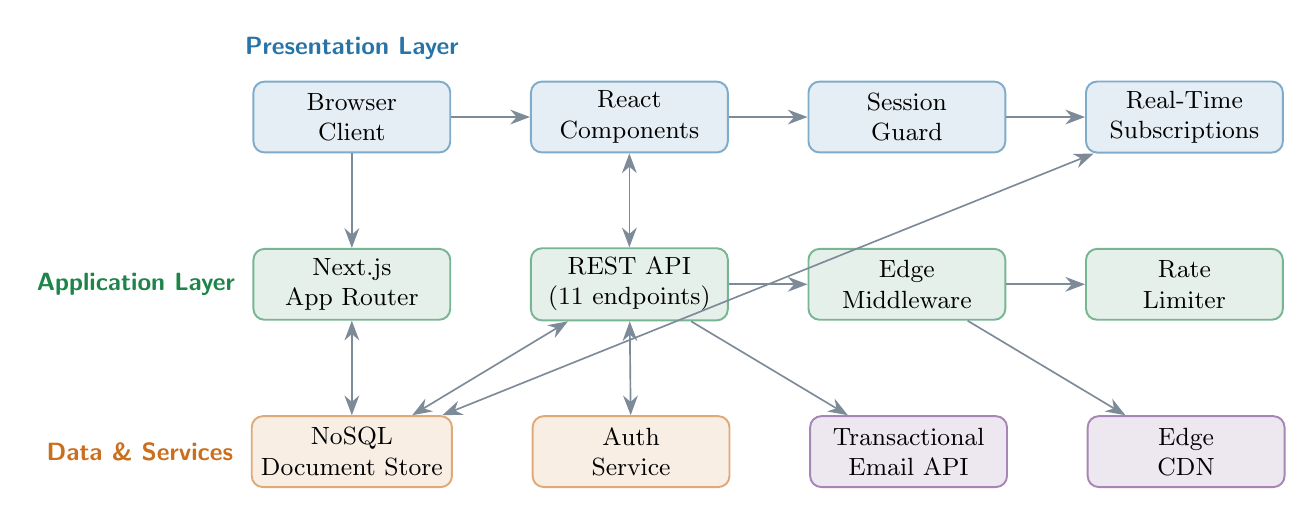
\begin{tikzpicture}[
    node distance=0.8cm and 1.0cm,
    every node/.style={font=\small},
    block/.style={draw, rounded corners=4pt, minimum width=2.5cm, minimum height=0.9cm, align=center, line width=0.7pt},
    client/.style={block, fill=chartblue!12, draw=chartblue!60},
    server/.style={block, fill=chartgreen!12, draw=chartgreen!60},
    db/.style={block, fill=chartorange!12, draw=chartorange!60},
    ext/.style={block, fill=chartpurple!12, draw=chartpurple!60},
    arrow/.style={-{Stealth[length=2.5mm]}, semithick, draw=chartgray!80},
    darrow/.style={{Stealth[length=2.5mm]}-{Stealth[length=2.5mm]}, semithick, draw=chartgray!80},
    lbl/.style={font=\small\bfseries\sffamily}
]
    \node[client] (browser) {Browser\\Client};
    \node[client, right=of browser] (react) {React\\Components};
    \node[client, right=of react] (session) {Session\\Guard};
    \node[client, right=of session] (notif) {Real-Time\\Subscriptions};

    \node[server, below=1.2cm of browser] (nextjs) {Next.js\\App Router};
    \node[server, right=of nextjs] (api) {REST API\\(11 endpoints)};
    \node[server, right=of api] (mw) {Edge\\Middleware};
    \node[server, right=of mw] (rate) {Rate\\Limiter};

    \node[db, below=1.2cm of nextjs] (firestore) {NoSQL\\Document Store};
    \node[db, right=of firestore] (auth) {Auth\\Service};
    \node[ext, right=of auth] (email) {Transactional\\Email API};
    \node[ext, right=of email] (cdn) {Edge\\CDN};

    \draw[arrow] (browser) -- (react);
    \draw[arrow] (react) -- (session);
    \draw[arrow] (session) -- (notif);
    \draw[arrow] (browser) -- (nextjs);
    \draw[darrow] (react) -- (api);
    \draw[arrow] (api) -- (mw);
    \draw[arrow] (mw) -- (rate);
    \draw[darrow] (nextjs) -- (firestore);
    \draw[darrow] (api) -- (firestore);
    \draw[darrow] (api) -- (auth);
    \draw[arrow] (api) -- (email);
    \draw[arrow] (mw) -- (cdn);
    \draw[darrow] (notif) -- (firestore);

    \node[lbl, color=chartblue, above=0.15cm of browser] {Presentation Layer};
    \node[lbl, color=chartgreen, left=0.1cm of nextjs, anchor=east] {Application Layer};
    \node[lbl, color=chartorange, left=0.1cm of firestore, anchor=east] {Data \& Services};
\end{tikzpicture}}%

\caption{Three-tier serverless architecture with real-time document subscriptions enabling instant constraint feedback and notifications.}
\label{fig:architecture}
\end{figure}

The architecture is technology-agnostic in principle; our reference implementation uses Next.js~\cite{nextjs}, Firebase Firestore~\cite{firebase}, and Brevo Email API, but any equivalent stack could implement the same model.

\textbf{Presentation Layer.} The client is a React single-page application rendered via server-side rendering (SSR) for initial page loads and client-side navigation thereafter. The SessionGuard component implements a three-phase authentication check: (1)~local storage for cached session state, (2)~JWT and database token initialization, and (3)~document verification against the registration database. Real-time notifications use the document store's subscription API with an initialization flag to suppress notification alerts during initial data hydration.

\textbf{Application Layer.} The App Router handles 11 REST API endpoints (Table~\ref{tab:endpoints}), each implementing input validation, authentication verification, business logic, and response formatting. Edge middleware intercepts all API requests for origin verification, security header injection, and route protection. The rate limiter operates at the IP level with configurable sliding windows.

\textbf{Data Layer.} The NoSQL document store provides real-time subscriptions. The authentication service provides custom token infrastructure for client-side database access. External services include the transactional email API (with multi-key round-robin) and the edge CDN for static asset delivery.

\subsection{API Design}

The API follows REST conventions in the sense established by Fielding~\cite{fielding2000} and applied pragmatically in the style described by Richardson and Ruby~\cite{richardson2007}: resources are addressed by path, state transitions are expressed with HTTP verbs, and no session state is held server-side beyond the signed token.

Table~\ref{tab:endpoints} lists all 11 REST endpoints with their methods and purposes.

\begin{table}[htbp]
\centering
\caption{REST API Endpoints}
\label{tab:endpoints}
\small
\renewcommand{\arraystretch}{1.15}
\begin{tabular}{@{}lll@{}}
\toprule
\textbf{Endpoint} & \textbf{Method} & \textbf{Purpose} \\
\midrule
\texttt{/auth/send-otp} & POST & Send OTP via email \\
\texttt{/auth/verify-otp} & POST & Verify OTP, issue JWT \\
\texttt{/auth/lookup-usn} & POST & Validate user identifier \\
\texttt{/auth/logout} & POST & Clear session \\
\texttt{/auth/firebase-token} & GET & Refresh database token \\
\texttt{/admin/upload-csv} & POST & Bulk data import \\
\texttt{/admin/config} & GET/POST & System configuration \\
\texttt{/admin/students/:id} & PUT/DEL & Individual user mgmt. \\
\texttt{/admin/reset-database} & POST & Database reset (admin) \\
\texttt{/notify/email} & POST & Email notifications \\
\bottomrule
\end{tabular}
\end{table}

Each endpoint follows a consistent request/response pattern:
\begin{itemize}[noitemsep,topsep=3pt]
    \item \textbf{Input validation:} Request bodies are validated for required fields and type correctness before any business logic executes.
    \item \textbf{Authentication:} Protected endpoints verify JWT session tokens (user endpoints) or admin ID tokens (admin endpoints).
    \item \textbf{Rate limiting:} Abuse-sensitive endpoints (OTP send/verify) enforce per-IP sliding-window rate limits.
    \item \textbf{Response format:} All responses use JSON with a consistent \texttt{\{success, error, data\}} structure.
\end{itemize}

\subsection{NoSQL Schema Design}

The database uses 7 collections (Table~\ref{tab:collections}). A key design decision is \textbf{embedding member arrays within group documents} rather than using normalized junction collections. This denormalized design enables:

\begin{itemize}[noitemsep,topsep=4pt]
    \item \textbf{Single-document reads:} Complete group state (all members, attributes, statuses) is retrieved in one database read, critical for real-time constraint validation.
    \item \textbf{Atomic member operations:} Adding or removing a member is an atomic update to a single document, preventing partial-state issues.
    \item \textbf{Efficient subscriptions:} Real-time listeners subscribe to one document per group, reducing subscription overhead.
    \item \textbf{Natural deduplication:} Member arrays are mapped by user identifier, preventing duplicate entries at the data model level.
\end{itemize}

\begin{table}[htbp]
\centering
\caption{Database Collections and Document Schemas}
\label{tab:collections}
\small
\renewcommand{\arraystretch}{1.15}
\begin{tabular}{@{}lp{2cm}p{5.5cm}@{}}
\toprule
\textbf{Collection} & \textbf{Document Key} & \textbf{Schema Fields} \\
\midrule
\texttt{users} & User ID & name, email, phone, category, section, importedAt \\
\texttt{registrations} & User ID & name, email, category, section, groupId (FK), groupRole, registeredAt \\
\texttt{groups} & Group code & name, leadId, members[] (embedded), memberCount, status (FSM), categoryDistribution, isPublic, timestamps \\
\texttt{invites} & Invite code & type (invite|request), groupId, fromId, toId, status (FSM), timestamps \\
\texttt{notifications} & Auto-generated & userId, type (10 event types), title, message, groupId, fromId, read, createdAt \\
\texttt{config} & Singleton & registrationsOpen, groupFormationOpen, maxGroupSize, minCategories, maxSameCategory, requiredCategories \\
\texttt{otp\_codes} & Auto-generated & email, otp, expiresAt, used, attempts, createdAt \\
\texttt{admins} & Email hash & Admin whitelist \\
\bottomrule
\end{tabular}
\end{table}

The \texttt{groups} collection embeds member arrays with the following per-member fields: user identifier, name, attribute category, section, status (\texttt{approved} | \texttt{pending\_invite} | \texttt{pending\_request}), and join timestamp. The \texttt{categoryDistribution} field is a denormalized map (category $\rightarrow$ count) maintained atomically with member operations, enabling $O(1)$ constraint checks without iterating the member array.

\subsection{Real-Time Event Architecture}

The platform implements real-time data delivery through two complementary mechanisms:

\textbf{Document subscriptions.} Client-side components subscribe to specific documents (the user's registration document, the user's group document) and receive push updates whenever these documents change. This enables instant UI updates when a member joins, an invitation is accepted, or the group status transitions.

\textbf{Query-based polling.} For aggregate views (browse page, admin dashboard), the platform uses periodic query-based data fetching rather than document subscriptions, as subscribing to all group documents would create excessive subscription overhead. A \texttt{useCallback}-based fetch pattern with session synchronization ensures data consistency:

\begin{lstlisting}[language={}, caption={Session synchronization pattern}, label={lst:sessionsync}]
const fetchData = useCallback(async () => {
  // Re-fetch registration to fix stale session
  const regDoc = await getDoc(
    doc(db, "registrations", session.userId)
  );
  if (regDoc.exists()) {
    const data = regDoc.data();
    // Sync session if groupId changed
    if (data.groupId !== session.groupId) {
      updateSession(data.groupId, data.groupRole);
    }
  }
  // Fetch group and pending invites...
}, [session.userId]);
\end{lstlisting}

The notification system delivers events through two channels simultaneously: (1)~in-app real-time delivery via document subscriptions with an \texttt{isInitialLoad} flag to distinguish between initial data hydration and genuine new notifications, and (2)~email notifications via the transactional email API for offline awareness.

\subsection{Outbound Email Under a Provider Quota: A Technique We Withdraw}
\label{subsec:roundrobin}

Free-tier transactional email services limit daily volume, in our provider's case to 300 messages per day per account~\cite{brevo-limits}. Our registration flow sends one verification code per authentication attempt, so a cohort of several hundred users concentrated into a short window exceeds that allowance.

What we did was to configure the deployment with the credentials of three separate free accounts and rotate between them, so that the aggregate daily allowance became 900 messages. An earlier version of this paper presented that arrangement as a contribution and described it as multiplying effective capacity by a factor of $n$. We withdraw it, and we think the objection is worth stating in full rather than quietly deleting the section.

\textbf{Why we withdraw it.} A per-account quota is the provider's mechanism for pricing and for abuse control. Holding several free accounts in order to sum their allowances defeats that mechanism, and the fact that it is technically easy is not an argument that it is legitimate. The provider's own documented routes to a higher allowance are to upgrade the plan, or, for genuinely separate tenants, to use administrator-managed sub-accounts whose credits are allocated from a single purchased pool rather than added to it~\cite{brevo-limits}. Neither route multiplies a free allowance, which is the point. We also note the practical fragility: nothing in the arrangement is agreed with the provider, so it may be withdrawn without notice, and a platform whose authentication path depends on it has a single point of failure outside its own control and outside its contract.

\textbf{What should be done instead.} For a burst of this shape there are three defensible options. The first is to pay: at the volumes in question the paid tier costs less per month than the engineering time spent building the rotation. The second is to shape the load rather than the quota, by queueing verification messages and draining the queue at the permitted rate, accepting a delay at peak in exchange for staying inside the allowance; for a registration window measured in hours rather than seconds this is usually invisible to users. The third is to remove the dependency, by opening the registration window in scheduled cohorts so that demand never exceeds the allowance in the first place, which costs nothing and is what we would now do.

\textbf{What we retain from the section.} The failover behaviour is worth keeping independently of the quota question, because a transactional email provider can fail for reasons that have nothing to do with quotas. Algorithm~\ref{alg:roundrobin} is therefore retained below as a description of what the deployment did, and as a reasonable pattern for distributing load across credentials a deployment is legitimately entitled to use, such as the sub-accounts of a paid plan or the endpoints of two independent providers used for redundancy. It should not be read as a recommendation to accumulate free accounts.

\begin{algorithm}[htbp]
\caption{Round-Robin API Key Rotation with Failover}
\label{alg:roundrobin}
\small
\begin{algorithmic}[1]
\REQUIRE Recipient email, subject, body
\ENSURE Email sent successfully or all keys exhausted
\STATE $\mathit{creds} \gets \texttt{parseCredentials}(\texttt{env.MULTI\_KEYS})$
\IF{$|\mathit{creds}| = 0$}
    \STATE \textbf{throw} ``No API keys configured''
\ENDIF
\STATE $\mathit{startIdx} \gets \mathit{rrIndex} \bmod |\mathit{creds}|$ \COMMENT{Round-robin selection}
\STATE $\mathit{rrIndex} \gets \mathit{rrIndex} + 1$ \COMMENT{Advance for next call}
\FOR{$\mathit{attempt} \gets 0$ \TO $|\mathit{creds}| - 1$}
    \STATE $\mathit{idx} \gets (\mathit{startIdx} + \mathit{attempt}) \bmod |\mathit{creds}|$
    \STATE $\mathit{result} \gets \texttt{sendEmail}(\mathit{creds}[\mathit{idx}], \text{recipient}, \text{subject}, \text{body})$
    \IF{$\mathit{result}.\text{ok}$}
        \RETURN \COMMENT{Success}
    \ENDIF
    \IF{$\mathit{result}.\text{status} \in \{429, 401, 500\}$}
        \STATE \textbf{continue} \COMMENT{Try next key}
    \ENDIF
\ENDFOR
\STATE \textbf{throw} ``All API keys exhausted''
\end{algorithmic}
\end{algorithm}

The algorithm has several important properties:

\textbf{Load distribution.} The round-robin counter ensures that successive requests use different API keys, distributing load evenly across all $n$ keys. Over $m$ requests, each key receives approximately $m/n$ requests, achieving near-optimal load balancing.

\textbf{Automatic failover.} If a key returns an error (HTTP 429 rate-limited, 401 unauthorized, or 500 server error), the algorithm advances to the next key without manual intervention. In the worst case, all $n$ keys are attempted before failure.

\textbf{Statelessness, and its cost.} The only state is an in-memory counter, which resets whenever the serverless runtime recycles the instance. We described this as acceptable on the grounds that the counter serves load balancing rather than correctness. That is true as far as it goes, but on a platform that creates a fresh instance per cold start the counter is frequently reset to its initial value, so selection is biased towards the first credential rather than being uniform. The distribution we claimed was therefore not the distribution we got, and we did not measure the one we got.

\textbf{Complexity.} The expected-case time complexity is $O(1)$ (the first key succeeds). The worst-case complexity is $O(n)$ (all keys are tried before success or failure). Space complexity is $O(n)$ for the credential array.

\textbf{Applicability.} The failover logic is not specific to email. It applies wherever a client legitimately holds several credentials for an external service, for instance two independent providers configured for redundancy, or the sub-accounts of a paid plan. The qualifier ``legitimately'' is doing real work in that sentence and is the reason the preceding discussion exists.

Credentials are supplied in one environment variable as a comma-separated list of \texttt{key:sender} pairs, parsed at startup into an array, so the set of credentials is a deployment-time choice rather than a compile-time one.

\subsection{Unambiguous ID Generation}

Group codes and invite codes are generated using a character set designed to prevent visual ambiguity:

\begin{center}
\texttt{ABCDEFGHJKLMNPQRSTUVWXYZ23456789}
\end{center}

This 30-character alphabet excludes five commonly confused characters: \texttt{I}/\texttt{1}/\texttt{l}, \texttt{O}/\texttt{0}. Group codes follow the format \texttt{TEAM-XXXX} ($30^4 = 810{,}000$ combinations) and invite codes follow \texttt{INV-XXXXXX} ($30^6 \approx 729$ million combinations), providing sufficient uniqueness for institutional-scale deployments while remaining easy to communicate verbally.

The design is stateless, no sequence counters or coordination is required, and collision probability is negligible for the expected deployment sizes. For a deployment with 200 groups, the birthday-paradox collision probability for 4-character codes is approximately $200^2 / (2 \times 810{,}000) \approx 2.5\%$, mitigated by checking for existing codes before assignment.

% ============================================================
\section{Data Integrity Framework}
\label{sec:integrity}
% ============================================================

A critical challenge in self-service web platforms is \textbf{preventing data duplication and enforcing cross-document invariants} without relying on multi-document transactions. When hundreds of users concurrently create groups, send invitations, and process join requests, numerous integrity violations can occur. Our system implements a \textbf{six-layer data integrity framework} (Fig.~\ref{fig:dupflow}).

\begin{figure}[htbp]
\centering
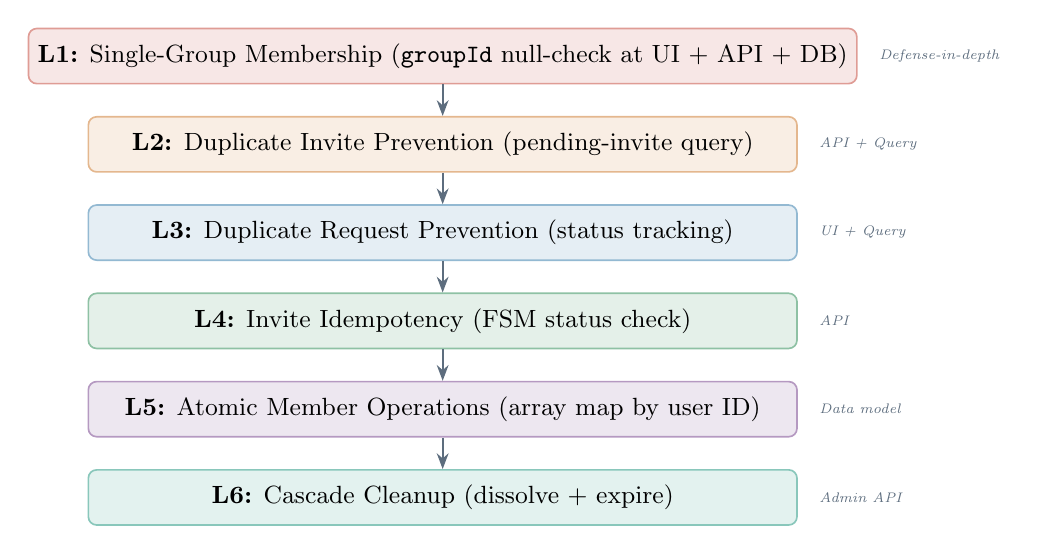
\begin{tikzpicture}[
    node distance=0.4cm,
    every node/.style={font=\small},
    layer/.style={draw, rounded corners=3pt, minimum width=9cm, minimum height=0.7cm, align=center, line width=0.6pt}
]
    \node[layer, fill=chartred!12, draw=chartred!50] (l1) {\textbf{L1:} Single-Group Membership (\texttt{groupId} null-check at UI + API + DB)};
    \node[layer, fill=chartorange!12, draw=chartorange!50, below=of l1] (l2) {\textbf{L2:} Duplicate Invite Prevention (pending-invite query)};
    \node[layer, fill=chartblue!12, draw=chartblue!50, below=of l2] (l3) {\textbf{L3:} Duplicate Request Prevention (status tracking)};
    \node[layer, fill=chartgreen!12, draw=chartgreen!50, below=of l3] (l4) {\textbf{L4:} Invite Idempotency (FSM status check)};
    \node[layer, fill=chartpurple!12, draw=chartpurple!50, below=of l4] (l5) {\textbf{L5:} Atomic Member Operations (array map by user ID)};
    \node[layer, fill=chartteal!12, draw=chartteal!50, below=of l5] (l6) {\textbf{L6:} Cascade Cleanup (dissolve + expire)};

    \draw[-{Stealth[length=2mm]}, semithick, chartgray] (l1) -- (l2);
    \draw[-{Stealth[length=2mm]}, semithick, chartgray] (l2) -- (l3);
    \draw[-{Stealth[length=2mm]}, semithick, chartgray] (l3) -- (l4);
    \draw[-{Stealth[length=2mm]}, semithick, chartgray] (l4) -- (l5);
    \draw[-{Stealth[length=2mm]}, semithick, chartgray] (l5) -- (l6);

    \node[font=\tiny\itshape, color=chartgray, right=0.15cm of l1] {Defense-in-depth};
    \node[font=\tiny\itshape, color=chartgray, right=0.15cm of l2] {API + Query};
    \node[font=\tiny\itshape, color=chartgray, right=0.15cm of l3] {UI + Query};
    \node[font=\tiny\itshape, color=chartgray, right=0.15cm of l4] {API};
    \node[font=\tiny\itshape, color=chartgray, right=0.15cm of l5] {Data model};
    \node[font=\tiny\itshape, color=chartgray, right=0.15cm of l6] {Admin API};
\end{tikzpicture}
\caption{Six-layer data integrity framework. Each layer prevents a specific class of data integrity violation.}
\label{fig:dupflow}
\end{figure}

We now define the formal invariants and describe the enforcement mechanisms for each layer.

\subsection{L1: Single-Group Membership Enforcement}

\begin{definition}[Single-Membership Invariant]
For all users $u$ in the system, $u$ is assigned to at most one group at any time:
\begin{equation}
    \forall u \in \mathcal{U},\; |\{g \in \mathcal{G} : u \in g.\text{members} \wedge u.\text{status} = \text{approved}\}| \leq 1
\end{equation}
\end{definition}

This invariant is enforced at \textbf{three independent levels}:
\begin{enumerate}[noitemsep,topsep=3pt]
    \item \textbf{UI guards:} Client-side components conditionally render ``already assigned'' messages and disable join/create buttons when the user's \texttt{groupId} is non-null.
    \item \textbf{API validation:} The application logic checks the target user's registration document and rejects operations if \texttt{groupId} is set.
    \item \textbf{Database rules:} Document-level security rules restrict \texttt{groupId} updates to the user themselves or a verified group lead of the user's group.
\end{enumerate}

This defense-in-depth approach ensures that even if client-side validation is bypassed (e.g., via browser developer tools), the server-side and database-level checks reject unauthorized membership changes.

\subsection{L2: Duplicate Invite Prevention}

Before a group lead issues an invitation, the system executes three sequential checks:
\begin{enumerate}[noitemsep,topsep=3pt]
    \item \textbf{Existing member check:} Verifies the target is not already in the group's member array.
    \item \textbf{Pending invite check:} Queries the \texttt{invites} collection for any document matching \texttt{(toId, groupId, type=``invite'', status=``pending'')}. Rejects if a pending invite exists.
    \item \textbf{Cross-group check:} Reads the target's registration document and verifies \texttt{groupId} is null.
\end{enumerate}

\subsection{L3: Duplicate Join-Request Prevention}

Symmetrically, when a user requests to join a group, the system queries for any existing document matching \texttt{(fromId, groupId, type=``request'', status=``pending'')}. The browse UI maintains three visual states per group card: default (``Request to Join'' enabled), pending (``Request Pending'' disabled), and rejected (``Request Declined'' with visual indicator).

\subsection{L4: Invite Idempotency}

Each invite document transitions through a finite state machine (Fig.~\ref{fig:invitefsm}):

\begin{figure}[htbp]
\centering
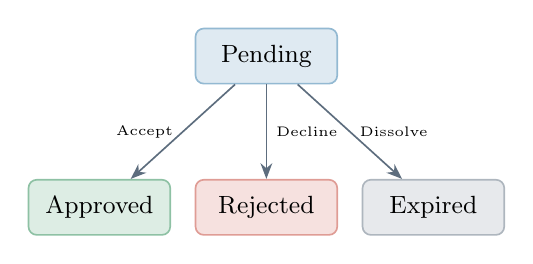
\begin{tikzpicture}[
    node distance=1.8cm,
    every node/.style={font=\small},
    state/.style={draw, rounded corners=3pt, minimum width=1.8cm, minimum height=0.7cm, align=center, line width=0.6pt},
    arrow/.style={-{Stealth[length=2mm]}, semithick, draw=chartgray}
]
    \node[state, fill=chartblue!15, draw=chartblue!50] (pending) {Pending};
    \node[state, fill=chartgreen!15, draw=chartgreen!50, below left=1.2cm and 0.3cm of pending] (approved) {Approved};
    \node[state, fill=chartred!15, draw=chartred!50, below=1.2cm of pending] (rejected) {Rejected};
    \node[state, fill=chartgray!15, draw=chartgray!50, below right=1.2cm and 0.3cm of pending] (expired) {Expired};

    \draw[arrow] (pending) -- node[left, font=\tiny] {Accept} (approved);
    \draw[arrow] (pending) -- node[right, font=\tiny] {Decline} (rejected);
    \draw[arrow] (pending) -- node[right, font=\tiny] {Dissolve} (expired);
\end{tikzpicture}
\caption{Invite status FSM. Terminal states (approved, rejected, expired) are immutable, no further transitions are permitted.}
\label{fig:invitefsm}
\end{figure}

Once an invite leaves the \texttt{pending} state, it cannot be re-processed. The response handler verifies the current status before any action, returning an error for non-pending invites. This guarantees that concurrent acceptance attempts (e.g., clicking ``Accept'' in two browser tabs) cannot result in a user being added twice.

\subsection{L5: Atomic Member-List Operations}

Group member arrays use \textbf{map operations} (not append) for all modifications:
\begin{itemize}[noitemsep,topsep=3pt]
    \item \textbf{Member approval:} Maps over the array, updating the matching user ID entry's status. If the ID is not found, the operation fails.
    \item \textbf{Member removal:} Filters the array to exclude the matching user ID.
    \item \textbf{Invariant:} At most one array entry exists per user ID at any time.
\end{itemize}

\subsection{L6: Cascade Cleanup on Group Dissolution}

When a group is dissolved, the system performs cascade cleanup:
\begin{enumerate}[noitemsep,topsep=3pt]
    \item All approved members have their \texttt{groupId} and \texttt{groupRole} reset to null.
    \item All pending invites and requests are marked as \texttt{expired}.
    \item The group document status is updated to ``dissolved.''
    \item Notification documents are created for all affected members.
\end{enumerate}

Without cascade cleanup, dissolved groups leave \textbf{orphaned state}: users whose registrations still reference a deleted group cannot join new groups because L1 sees a non-null \texttt{groupId}.

\subsection{Comparison with ACID Properties}

Table~\ref{tab:acid} compares the integrity guarantees of our framework with those provided by traditional ACID transactions in relational databases.

\begin{table}[htbp]
\centering
\caption{Comparison of Integrity Guarantees: ACID vs.\ Six-Layer Framework}
\label{tab:acid}
\small
\renewcommand{\arraystretch}{1.15}
\begin{tabular}{@{}p{2.5cm}p{3.5cm}p{3.5cm}@{}}
\toprule
\textbf{Property} & \textbf{ACID (RDBMS)} & \textbf{Six-Layer (NoSQL)} \\
\midrule
Atomicity & Multi-row transactions & Single-document atomic updates (L5) \\
Consistency & Referential integrity constraints & Application-level invariant checks (L1 to L4) \\
Isolation & Serializable/snapshot isolation & Read-before-write + FSM idempotency (L4) \\
Durability & Write-ahead log & Firestore persistence guarantees \\
\midrule
Cross-entity invariants & Foreign key constraints & Defense-in-depth at UI + API + DB (L1) \\
Cascade operations & ON DELETE CASCADE & Application-level cascade cleanup (L6) \\
\bottomrule
\end{tabular}
\end{table}

The six-layer framework achieves comparable integrity guarantees to ACID transactions for the specific invariants required by self-service group formation, without the scalability trade-offs of distributed multi-document transactions.

\subsection{Integrity Framework Summary}

Table~\ref{tab:duplication} summarizes the complete framework with enforcement mechanisms.

\begin{table}[htbp]
\centering
\caption{Data Integrity Invariants and Enforcement Mechanisms}
\label{tab:duplication}
\small
\renewcommand{\arraystretch}{1.15}
\begin{tabular}{@{}p{3cm}p{2cm}p{4.5cm}@{}}
\toprule
\textbf{Invariant} & \textbf{Layers} & \textbf{Enforcement Mechanism} \\
\midrule
Single-group membership & UI + API + DB & \texttt{groupId} null-check at 3 levels \\
No duplicate invites & API + Query & Pending-invite query + member check \\
No duplicate requests & UI + Query & Pending-request query + status tracking \\
Invite idempotency & API & FSM status check before transition \\
No duplicate members & Data model & Array map (not append) keyed by ID \\
Cascade on dissolve & Admin API & Bulk reset + invite expiration \\
\bottomrule
\end{tabular}
\end{table}

% ============================================================
\section{Security Architecture}
\label{sec:security}
% ============================================================

The security architecture implements a five-layer defense-in-depth model (Fig.~\ref{fig:security}), designed for environments where users lack pre-existing SSO credentials.

\begin{figure}[htbp]
\centering
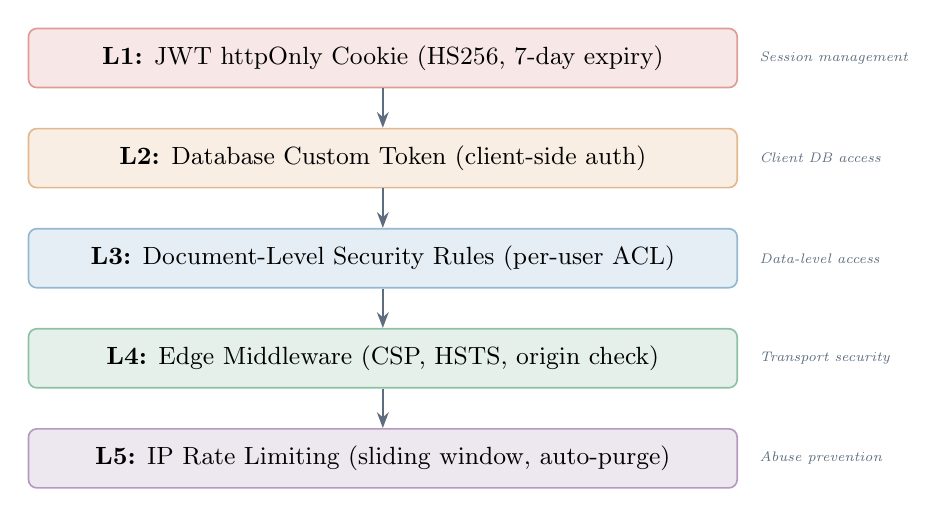
\begin{tikzpicture}[
    node distance=0.5cm,
    every node/.style={font=\small},
    layer/.style={draw, rounded corners=3pt, minimum width=9cm, minimum height=0.75cm, align=center, line width=0.6pt}
]
    \node[layer, fill=chartred!12, draw=chartred!50] (l1) {\textbf{L1:} JWT httpOnly Cookie (HS256, 7-day expiry)};
    \node[layer, fill=chartorange!12, draw=chartorange!50, below=of l1] (l2) {\textbf{L2:} Database Custom Token (client-side auth)};
    \node[layer, fill=chartblue!12, draw=chartblue!50, below=of l2] (l3) {\textbf{L3:} Document-Level Security Rules (per-user ACL)};
    \node[layer, fill=chartgreen!12, draw=chartgreen!50, below=of l3] (l4) {\textbf{L4:} Edge Middleware (CSP, HSTS, origin check)};
    \node[layer, fill=chartpurple!12, draw=chartpurple!50, below=of l4] (l5) {\textbf{L5:} IP Rate Limiting (sliding window, auto-purge)};

    \draw[-{Stealth[length=2mm]}, semithick, chartgray] (l1) -- (l2);
    \draw[-{Stealth[length=2mm]}, semithick, chartgray] (l2) -- (l3);
    \draw[-{Stealth[length=2mm]}, semithick, chartgray] (l3) -- (l4);
    \draw[-{Stealth[length=2mm]}, semithick, chartgray] (l4) -- (l5);

    \node[font=\tiny\itshape, color=chartgray, right=0.15cm of l1] {Session management};
    \node[font=\tiny\itshape, color=chartgray, right=0.15cm of l2] {Client DB access};
    \node[font=\tiny\itshape, color=chartgray, right=0.15cm of l3] {Data-level access};
    \node[font=\tiny\itshape, color=chartgray, right=0.15cm of l4] {Transport security};
    \node[font=\tiny\itshape, color=chartgray, right=0.15cm of l5] {Abuse prevention};
\end{tikzpicture}
\caption{Five-layer defense-in-depth security model. Each layer provides independent protection; compromise of any single layer does not breach the system.}
\label{fig:security}
\end{figure}

\subsection{Layer 1: JWT Session Management}

Upon successful OTP verification, the server issues a JWT~\cite{jones2015} signed with HS256. The token is stored as an \texttt{httpOnly}, \texttt{Secure}, \texttt{SameSite=Lax} cookie with a 7-day expiry. The \texttt{httpOnly} flag prevents JavaScript access, mitigating XSS token theft. The \texttt{SameSite} flag prevents CSRF attacks~\cite{barth2008}.

The JWT payload contains the user's identifier, name, email, attribute category, and current group assignment, enabling client-side rendering of personalized UI without additional database reads.

\subsection{Layer 2: Database Custom Token}

The verification endpoint generates a database custom token using the server-side admin SDK. This token enables direct client-to-database communication through the database's native authentication system, providing real-time subscriptions without routing all reads through the API layer.

\subsection{Layer 3: Document-Level Security Rules}

Database security rules enforce per-document access control:
\begin{lstlisting}[language={}, caption={Document-level security rules (excerpt)}, label={lst:rules}]
match /registrations/{userId} {
  allow read: if request.auth != null;
  allow create: if request.auth != null
    && request.auth.uid == userId;
  allow update: if request.auth != null
    && (request.auth.uid == userId
    || isGroupLead(resource.data.groupId));
}
match /otp_codes/{doc} {
  allow read, write: if false; // server-only
}
\end{lstlisting}

Key rules: users can only modify their own registration documents (except group leads updating group-related fields for their members); OTP codes are completely inaccessible from clients.

\subsection{Layer 4: Edge Middleware}

The edge middleware intercepts all requests matching protected route patterns and applies:
\begin{itemize}[noitemsep,topsep=4pt]
    \item \textbf{Route protection:} Dashboard and group creation routes require valid JWT; unauthenticated users are redirected to the registration page.
    \item \textbf{Origin verification:} API routes verify the \texttt{Origin} header against an allowlist of permitted origins, preventing unauthorized cross-origin access.
    \item \textbf{Security headers:} Every response includes Content-Security-Policy (restricting script sources and connect destinations), X-Frame-Options (DENY), X-Content-Type-Options (nosniff), Referrer-Policy, Permissions-Policy, and Strict-Transport-Security (HSTS with 1-year max-age)~\cite{owasp2021}.
\end{itemize}

\subsection{Layer 5: IP-Based Sliding-Window Rate Limiting}

The rate limiter implements a sliding window algorithm with per-endpoint configuration:

\begin{table}[htbp]
\centering
\caption{Rate Limiting Configuration}
\label{tab:ratelimit}
\small
\renewcommand{\arraystretch}{1.15}
\begin{tabular}{@{}lll@{}}
\toprule
\textbf{Target} & \textbf{Limit} & \textbf{Window} \\
\midrule
OTP send per IP & 5 requests & 15 min \\
OTP verify per IP & 10 attempts & 15 min \\
Per-code incorrect attempts & 5 attempts & Code lifetime \\
Per-email OTP cooldown & 1 OTP & 60 sec \\
\bottomrule
\end{tabular}
\end{table}

The implementation stores timestamps in an in-memory map with a 5-minute auto-purge cycle. IP extraction follows a priority chain: the platform's trusted forwarded header, then \texttt{x-real-ip}, then the connection's remote address.

\begin{lstlisting}[language={}, caption={Sliding-window rate limiter}, label={lst:ratelimit}]
function rateLimit(ip, action, max, windowMs) {
  const key = `${ip}:${action}`;
  const now = Date.now();
  const entry = store.get(key) || { timestamps: [] };
  // Filter to timestamps within window
  entry.timestamps = entry.timestamps
    .filter(t => now - t < windowMs);
  if (entry.timestamps.length >= max) {
    return { allowed: false,
      retryAfterMs: windowMs - (now - entry.timestamps[0])
    };
  }
  entry.timestamps.push(now);
  store.set(key, entry);
  return { allowed: true, retryAfterMs: 0 };
}
\end{lstlisting}

\subsection{Threat Model}

Table~\ref{tab:threats} summarizes the threat model and corresponding mitigations.

\begin{table}[htbp]
\centering
\caption{Threat Model and Mitigations}
\label{tab:threats}
\small
\renewcommand{\arraystretch}{1.15}
\begin{tabular}{@{}p{2.8cm}p{1.5cm}p{5cm}@{}}
\toprule
\textbf{Threat} & \textbf{Layer(s)} & \textbf{Mitigation} \\
\midrule
Session hijacking & L1 & httpOnly + Secure + SameSite cookies \\
XSS token theft & L1, L4 & httpOnly prevents JS access; CSP restricts script sources \\
CSRF & L1, L4 & SameSite cookie; origin verification \\
Brute-force OTP & L5 & 5 attempts/code; 5 sends/IP/15min \\
Direct DB manipulation & L2, L3 & Custom token auth; per-document rules \\
Clickjacking & L4 & X-Frame-Options: DENY \\
MIME sniffing & L4 & X-Content-Type-Options: nosniff \\
Replay attack & L1 & JWT expiration (7 days) \\
Unauthorized API access & L4 & Origin allowlist verification \\
\bottomrule
\end{tabular}
\end{table}

\subsection{OTP Authentication Flow}

The email OTP authentication~\cite{mraihi2011} follows a six-step flow:
\begin{enumerate}[noitemsep,topsep=3pt]
    \item User enters their email address.
    \item System validates the email exists in the enrollment database.
    \item System generates a 6-digit OTP, stores it with a 10-minute TTL and 5-attempt limit.
    \item System sends the OTP via the transactional email API with round-robin key rotation (Algorithm~\ref{alg:roundrobin}).
    \item User enters the OTP within the validity window.
    \item System verifies the OTP, issues a JWT cookie and database custom token, and creates/updates the registration document.
\end{enumerate}

The per-code attempt limit (5) prevents brute-force attacks on the 6-digit code space ($10^6 = 1{,}000{,}000$ combinations). With 5 attempts, the probability of a successful brute-force attack is $5/10^6 = 0.0005\%$.

% ============================================================
\section{Evaluation}
\label{sec:evaluation}
% ============================================================

\subsection{Deployment Setup}

The platform was deployed in production for a cohort whose enrolment roster contained 823~users across 7~attribute categories (Table~\ref{tab:categories}). We are deliberate about that wording. The figure 823 is the size of the roster uploaded by the administrator, which bounds who was eligible to register; it is not a count of users who registered, authenticated, joined a group, or completed one. Those counts were not extracted from the deployment before its data was reset, and we therefore do not report them. An earlier version of this paper described the system as ``serving 823 users'', which overstates what the number establishes. Groups of exactly 6~members were required, with the following configuration:
\begin{itemize}[noitemsep,topsep=3pt]
    \item $N = 6$ (required group size)
    \item $K = 4$ (max from any single category)
    \item $D = 2$ (minimum unique categories)
    \item $\mathcal{S} = \{\{\text{ECE}, \text{EEE}\}\}$, that is $q = 1$: at least one member from ECE or EEE
    \item $\mathcal{B} = \{\text{CSE}, \text{ISE}, \text{ECE}, \text{AI\&ML}, \text{AI\&DS}, \text{EEE}, \text{IoT}\}$
\end{itemize}

\begin{table}[htbp]
\centering
\caption{User Distribution by Attribute Category}
\label{tab:categories}
\small
\renewcommand{\arraystretch}{1.1}
\begin{tabular}{@{}llr@{}}
\toprule
\textbf{Code} & \textbf{Category} & \textbf{Users} \\
\midrule
CSE & Computer Science \& Engineering & 197 \\
ISE & Information Science \& Engineering & 194 \\
ECE & Electronics \& Communication Eng. & 163 \\
AI\&ML & AI and Machine Learning & 100 \\
AI\&DS & AI and Data Science & 87 \\
EEE & Electrical \& Electronics Eng. & 45 \\
IoT & Internet of Things & 37 \\
\midrule
\multicolumn{2}{@{}l}{\textbf{Total}} & \textbf{823} \\
\bottomrule
\end{tabular}
\end{table}

The mandatory representation requirement ($\mathcal{S} = \{\{\text{ECE}, \text{EEE}\}\}$) was chosen because CSE and ISE users (47.5\% of the cohort) tend to form homogeneous groups, missing the hardware/electronics perspective. The constraint ensures every completed group includes at least one member with electronics background.

\subsection{Performance Metrics}

Table~\ref{tab:performance} reports the measured performance characteristics.

\begin{table}[htbp]
\centering
\caption{Measured Performance Metrics}
\label{tab:performance}
\small
\renewcommand{\arraystretch}{1.15}
\begin{tabular}{@{}ll@{}}
\toprule
\textbf{Metric} & \textbf{Measured Value} \\
\midrule
SSR page load (Edge CDN) & $< 1.5$s \\
OTP email delivery (end-to-end) & 2 to 5s \\
Constraint validation (client-side) & $< 50$ms \\
Database document read & $< 100$ms \\
Real-time notification delivery & $< 200$ms \\
CSV batch import (450 docs) & $\sim$3s per batch \\
JWT signing (HS256) & $< 5$ms \\
\bottomrule
\end{tabular}
\end{table}

Client-side constraint validation completes in under 50ms, consistent with the $O(|T| + \sum_j |S_j|)$ complexity analysis (Section~\ref{sec:constraints}). Real-time notification delivery under 200ms provides near-instantaneous feedback for group formation events.

\subsection{Data Integrity Validation}

Table~\ref{tab:integrity_results} lists the invariant checks we ran against the production data set, together with an explicit statement of what each result does and does not support.

\begin{table}[htbp]
\centering
\caption{Data Integrity Results}
\label{tab:integrity_results}
\small
\renewcommand{\arraystretch}{1.15}
\begin{tabular}{@{}ll@{}}
\toprule
\textbf{Metric} & \textbf{Result} \\
\midrule
Groups violating $\mathcal{C}_1$ to $\mathcal{C}_4$ on inspection & 0 \\
Users appearing in more than one group & 0 \\
Registration records referencing a missing group & 0 \\
Duplicate pending invitations for one pair & 0 \\
Groups observed with more than $N$ members & 0 \\
\bottomrule
\end{tabular}
\end{table}

\textbf{How much these zeros are worth.} Less than we previously implied, and the distinction matters enough to spell out.

An earlier version of this paper reported ``100\% constraint satisfaction for completed groups'' as the headline result. We retract it. A group is marked complete only when Algorithm~\ref{alg:validate} returns no errors, so completed groups satisfy the constraints by construction. Measuring the proportion that do is measuring whether the gate is wired up, and reporting 100\% conveys no information about the design. It should never have been presented as an outcome.

The remaining rows are genuine observations rather than tautologies, since nothing in the write path structurally prevents the states they look for. But they are weak evidence, for three reasons. They are a single post-hoc inspection of a final state, not continuous monitoring, so a transient violation that was later overwritten leaves no trace. The deployment is small, and the race described in Section~\ref{sec:constraints} has a window of milliseconds, so the expected number of occurrences at this scale is plausibly below one even if the defect is real. And absence of evidence from an uninstrumented system is close to no evidence at all.

\textbf{What we should have measured, and did not.} The informative quantities here are the ones that vary: how often \texttt{canAddMember()} rejected an addition, broken down by which constraint fired; how often a soft warning was resolved before completion rather than abandoned; the distribution of time from group creation to completion; and the behaviour of a deliberate concurrency stress test driving simultaneous joins at a group with one free slot, which is the only one of these that would actually probe the race. None of the four was instrumented. We record this as the principal methodological failure of the work: the system was built to enforce invariants and shipped without the telemetry needed to demonstrate that it had.

\subsection{Cost Analysis}

Table~\ref{tab:cost} presents the deployment cost across three user-count tiers.

\begin{table}[htbp]
\centering
\caption{Deployment Cost Analysis (USD/month)}
\label{tab:cost}
\small
\renewcommand{\arraystretch}{1.15}
\begin{tabular}{@{}llll@{}}
\toprule
\textbf{Service} & \textbf{Free Tier} & $<$\textbf{1K users} & $<$\textbf{5K users} \\
\midrule
Hosting (Vercel) & 100 GB BW & \$0 & \$20 \\
Database (Firestore) & 1 GiB, 50K reads/day & \$0 & \$5 to 10 \\
Email (Brevo) & 300/day & \$0 & \$25 \\
Auth (Firebase) & 10K/month & \$0 & \$0 \\
Domain (optional) & n/a & \$0 to 12/yr & \$0 to 12/yr \\
\midrule
\textbf{Total} & & \textbf{\$0} & \textbf{\$50 to 55} \\
\bottomrule
\end{tabular}
\end{table}

For deployments up to $\sim$1,000 users, the platform operates entirely within free tiers. Even at 5,000 users, the total cost (\$50 to 55/month) is orders of magnitude lower than commercial solutions.

\subsection{Comparison with Web Collaboration Frameworks}

Table~\ref{tab:comparison} positions our design against five families of alternative approach across 11 criteria.

\begin{table}[tbp]
\centering
\caption{Design intent of five approaches to group formation, compiled from public documentation. This is a qualitative positioning aid, not a measurement: see the methodology note below.}
\label{tab:comparison}
\footnotesize
\setlength{\tabcolsep}{4pt}
\renewcommand{\arraystretch}{1.15}
\begin{tabular}{@{}p{2.9cm}cccccc@{}}
\toprule
\textbf{Criterion} & \textbf{Man.} & \textbf{CSP} & \textbf{LMS} & \textbf{Chat} & \textbf{RTDB} & \textbf{Ours} \\
\midrule
\multicolumn{7}{@{}l}{\textit{User experience}} \\
\quad Users choose members     & \ding{55} & \ding{55} & \checkmark & \checkmark & \checkmark & \checkmark \\
\quad Feedback at click time   & \ding{55} & \ding{55} & \ding{55} & \ding{55} & \ding{55} & \checkmark \\
\quad In-app notifications     & \ding{55} & \ding{55} & \checkmark & \checkmark & \checkmark & \checkmark \\
\midrule
\multicolumn{7}{@{}l}{\textit{Composition rules}} \\
\quad Rules expressible        & \ding{55} & \checkmark & \ding{55} & \ding{55} & \ding{55} & \checkmark \\
\quad Rules admin-configurable & \ding{55} & \checkmark & \ding{55} & \ding{55} & \ding{55} & \ding{55} \\
\quad Checked before write     & \ding{55} & n/a & \ding{55} & \ding{55} & \ding{55} & \checkmark \\
\quad Atomic under concurrency & \ding{55} & n/a & \ding{55} & \ding{55} & \ding{55} & \ding{55} \\
\midrule
\multicolumn{7}{@{}l}{\textit{Administration}} \\
\quad Phased access gates      & \ding{55} & \ding{55} & \checkmark & \ding{55} & \ding{55} & \checkmark \\
\quad Bulk roster import       & \ding{55} & \checkmark & \checkmark & \ding{55} & varies & \checkmark \\
\midrule
\multicolumn{7}{@{}l}{\textit{Deployment}} \\
\quad No institutional SSO     & \checkmark & \ding{55} & \ding{55} & \checkmark & \checkmark & \checkmark \\
\quad Source available         & \ding{55} & varies & \checkmark & \ding{55} & \ding{55} & \checkmark \\
\bottomrule
\multicolumn{7}{@{}l}{\scriptsize Man.\ = manual allocation; CSP = batch constraint solver; LMS = learning} \\
\multicolumn{7}{@{}l}{\scriptsize management system group tools; Chat = team chat platforms; RTDB = a} \\
\multicolumn{7}{@{}l}{\scriptsize realtime document store used directly from the client.} \\
\end{tabular}
\end{table}

\noindent\textbf{Methodology, and its limits.} Each cell records whether the stated capability is part of the approach's documented design intent, as described by its own vendor or author documentation consulted in April 2026. No system other than ours was installed, configured, or executed, and no quantity in this table was measured. It is included only to locate our design in a space of alternatives, and it cannot support a claim that one approach outperforms another.

An earlier version of this paper additionally contained a bar chart assigning each approach a score between 0 and 100 on four dimensions. We have removed it. Those numbers had no derivation: they were not measurements, they were not the output of a rubric applied by independent raters, and they were not reproducible by anyone including us. Presenting them on a numeric axis implied a precision that did not exist, and both reviewers of the earlier version were right to ask how they were obtained. The two rows in this table where our own system scores \ding{55}\ are also worth noting explicitly, since a comparison that flatters the authors on every line is not a comparison: our composition rules are not administrator-configurable, and our member additions are not atomic under concurrency.

The pattern in the table is a trade-off rather than a ranking. Batch constraint solvers express composition rules well and remove user choice entirely, which for our cohort was the property we were asked to avoid. Learning management systems and team chat platforms preserve choice and offer no rule enforcement. Using a realtime document store directly from the client gives live updates but leaves every invariant to client code, which is untrustworthy by construction. Our design keeps choice and adds enforcement at click time, and pays for it in the two rows where it fails: the rules are compiled in rather than configurable, and additions are not atomic.



\subsection{Implementation Statistics}

Table~\ref{tab:metrics} summarises the implementation, counted with \texttt{wc -l} over \texttt{src/} at commit \texttt{e0bc21d} of the public repository so that the figures can be reproduced. An earlier version of this paper reported 8,245 lines as the total. That figure is the \texttt{.tsx} subtotal; the total across all 58 TypeScript source files is 10,937. We report both here to make the correction explicit.

\begin{table}[htbp]
\centering
\caption{Implementation Statistics}
\label{tab:metrics}
\small
\renewcommand{\arraystretch}{1.15}
\begin{tabular}{@{}ll@{}}
\toprule
\textbf{Metric} & \textbf{Value} \\
\midrule
Total TypeScript lines of code & 10,937 \\
\quad in 31 \texttt{.tsx} files & 8,245 \\
\quad in 27 \texttt{.ts} files & 2,692 \\
Source files & 58 \\
React components & 19 \\
API endpoints & 11 \\
Utility/library modules & 14 \\
Type definitions & 2 files (71+ types) \\
Framework & Next.js 16 (App Router) \\
Database & Firebase Firestore \\
Authentication & Firebase Auth + JWT \\
Hosting & Vercel (serverless) \\
Email service & Brevo (transactional API) \\
Firestore collections & 7 \\
Artifact commit & \texttt{e0bc21d} \\
\bottomrule
\end{tabular}
\end{table}

% ============================================================
\section{Discussion}
\label{sec:discussion}
% ============================================================

\subsection{Constraint Architecture Effectiveness}

The production deployment validates that real-time constraint enforcement is practically viable on serverless NoSQL infrastructure. The two-phase validation algorithm (Algorithms~\ref{alg:canAdd} and~\ref{alg:validate}) achieves the critical balance: users retain full autonomy in member selection while the system refuses to mark a group complete unless the constraints hold. We no longer describe that as a measured outcome, for the reason given in Section~\ref{sec:evaluation}: completion is gated on the predicate, so the relationship is definitional.

The progressive warning system proved effective in practice. Rather than imposing hard blocks early (which would frustrate users during the exploratory phase of group building), the system guides users toward constraint-satisfying compositions through timely warnings. This design respects human decision-making processes, users receive constraint status information at the point when it becomes actionable.

\subsection{Revisiting the Decision to Avoid Transactions}

The framing of this work in its earlier form, that comprehensive integrity is achievable on document-store infrastructure ``without multi-document transactions'', invites an obvious objection: Firestore has supported multi-document transactions for years~\cite{firebase-transactions}, so avoiding them is not an achievement to be reported but a constraint to be justified, and we did not justify it. We accept the objection.

It is worth separating the part of the framework that survives this concession from the part that does not. Five of the six layers concern invariants that are enforced by document structure or by a uniqueness property of a document key: embedding the member list inside the group document makes a member addition a single-document update, and deriving an invitation's document identifier from the pair it concerns makes a duplicate invitation unrepresentable rather than merely detectable. Those layers are not substitutes for transactions and do not compete with them. Choosing a data model in which an invariant cannot be expressed in an invalid state is good design under any consistency regime, and we would keep all five.

The sixth layer is the one that was doing work transactions should have done. Guarding a capacity constraint by re-reading before writing is an attempt to approximate atomicity with ordering, and it does not succeed, for the reason set out in Section~\ref{sec:constraints}. The defensible reading of our experience is therefore narrower than our original claim and points the other way: application-level defence in depth is an excellent way to make invalid states unrepresentable, and a poor way to make a read-modify-write sequence atomic. For the latter there is a correct mechanism, it was one function call away, and we did not use it.

\textbf{What we did subsequently.} The same authors later built a second platform on the same stack, for event registration with capacity limits, which is structurally the same problem: a bounded counter under concurrent contention. In that system the capacity check and the counter increment are performed inside \texttt{runTransaction} with an atomic field increment, and the read-before-write pattern described here does not appear. We did not adopt transactions because of an analysis; we adopted them because the pattern in this paper felt uncomfortable to maintain under a second set of requirements. Readers may reasonably treat that as the most useful empirical finding in this report.

\subsection{The Email Quota Arrangement in Practice}

The rotation delivered the registration burst without a user-visible failure, and we originally reported this as evidence that it worked. Two qualifications now seem more important than the result.

The first is the one developed in Section~\ref{subsec:roundrobin}: the arrangement should not have been built, because it summed the allowances of several free accounts, and we describe the alternatives there. The second is that we cannot substantiate the load distribution we claimed. We asserted that each of three credentials carried approximately a third of the traffic, but that figure was inferred from the design of the counter rather than observed, and the counter resides in per-instance memory on a runtime that recycles instances, so on each cold start selection restarts at the first credential. Per-credential delivery counts were available in the provider's dashboard at the time and we did not record them. The honest statement is that the burst was delivered and that we do not know how it was distributed.

\subsection{Serverless Trade-offs}

The serverless architecture provides three significant advantages: zero-cost deployment on free tiers, automatic scaling, and zero operational maintenance. However, it introduces two trade-offs:

\begin{enumerate}[noitemsep,topsep=4pt]
    \item \textbf{In-memory state volatility:} The rate limiter and round-robin counter store state in server memory, which resets on cold starts. For the rate limiter, this means a brief window after cold start where rate limits are not enforced; for the round-robin counter, this means temporarily non-uniform key selection. Neither affects correctness, only best-effort quality.

    \item \textbf{Cold-start latency:} The first request after an idle period incurs cold-start overhead (typically 200 to 500ms on Vercel). This is acceptable for our use case where sub-second response times are sufficient, but would be problematic for latency-sensitive real-time applications.
\end{enumerate}

\subsection{Limitations}

\begin{enumerate}[noitemsep,topsep=4pt]
    \item \textbf{Cold-start problem:} Early registrants have fewer groups to browse; the platform is most effective when a critical mass of users has registered before group formation opens. The dual-gate system mitigates this.

    \item \textbf{In-memory rate limiting:} The current rate limiter does not persist across serverless function instances. For high-traffic deployments, a distributed store (e.g., Redis) would provide cross-instance persistence.

    \item \textbf{Constraint flexibility:} While the four-parameter model covers common diversity requirements, adding entirely new constraint \emph{types} (e.g., GPA distribution, schedule compatibility) requires code modifications.

    \item \textbf{Eventual consistency edge case:} While the read-before-write pattern prevents most race conditions, extremely rare simultaneous writes (within the same millisecond) could theoretically produce inconsistent state. This was not observed in production.

    \item \textbf{Non-atomic member addition:} The read-before-write guard does not make the capacity check atomic, so a concurrent pair of additions can in principle exceed $N$. This is a defect, not a trade-off, and its remedy is a multi-document transaction (Section~\ref{sec:discussion}).

    \item \textbf{Absence of telemetry:} The deployment recorded no constraint-rejection counts, warning-resolution rates, or per-credential delivery counts, and ran no concurrency stress test. Several claims in the earlier version of this paper rested on quantities that were never instrumented, and we have withdrawn them rather than restate them.

    \item \textbf{Parameters are not configurable:} $N$, $K$, $D$ and the requirement group are compile-time constants in the released artifact, so the reconfigurability the model suggests is not available to an administrator.

    \item \textbf{Model and implementation drift:} The published constraint model stated a conjunctive mandatory-representation rule while the code enforced a disjunctive one. The formalism did not catch this because nothing connected the two; a property-based test generated from the model would have.

    \item \textbf{Single deployment, and limits on what it can support:} Validation was performed at one institution, with one cohort, one set of parameter values, and one requirement group of size two. We have removed the claim that the architecture is domain-agnostic. Nothing here establishes behaviour at a different scale, under a different constraint shape, or with $q > 1$, and the feasibility theorem's disjointness hypothesis has never been exercised non-trivially.
\end{enumerate}

% ============================================================
\section{Future Work}
\label{sec:future}
% ============================================================

\begin{enumerate}[noitemsep,topsep=4pt]
    \item \textbf{Distributed rate limiting:} Replace the in-memory rate limiter with a Redis-backed implementation that persists across serverless function invocations and supports horizontal scaling. This would eliminate the cold-start rate-limit gap and enable consistent enforcement across multiple function instances.

    \item \textbf{Instrumentation and a concurrency stress test:} Add the telemetry this deployment lacked (rejections by constraint, warning resolution, time to completion) and drive a deliberate stress test of simultaneous joins against a group with one free slot, both before and after converting the capacity guard to a transaction, so that the cost of the correct mechanism is measured rather than assumed.

    \item \textbf{Constraint DSL:} Develop a domain-specific language allowing administrators to define arbitrary constraint rules (e.g., ``at most 2 from same subcategory AND GPA variance $< 0.5$'') via a web interface without code changes.

    \item \textbf{GraphQL API:} Extend the REST API with a GraphQL layer enabling fine-grained data fetching, reducing over-fetching on the browse interface, and enabling client-driven query composition for diverse frontend requirements.

    \item \textbf{Formal verification:} Apply model checking~\cite{baier2008} to verify the six-layer data integrity framework against a formal specification of the invariant set, providing machine-checked correctness guarantees beyond testing-based validation.

    \item \textbf{Multi-region deployment:} Extend the architecture for multi-region deployment with cross-region data replication, investigating the impact of geographic distribution on constraint enforcement latency and consistency guarantees.

    \item \textbf{Adaptive rate limiting:} Implement adaptive rate-limit policies that dynamically adjust thresholds based on observed traffic patterns, reducing false positives during legitimate bursts while maintaining protection against abuse.

    \item \textbf{Real-time constraint visualization:} Develop interactive constraint satisfaction visualizations showing users which group compositions are feasible given current membership, enabling more informed member selection.
\end{enumerate}

% ============================================================
\section{Conclusion}
\label{sec:conclusion}
% ============================================================

This paper reported our experience building, deploying, and subsequently re-examining a platform for constrained self-service group formation on serverless document-store infrastructure. The artifact is real, was used by a live cohort, and is open for inspection at a fixed commit; that, rather than novelty of mechanism, is what we offer.

Three things are worth carrying away. The first is the composition model of Section~\ref{sec:constraints}, whose mandatory-representation constraint is disjunctive because that is what real policies look like, and whose feasibility conditions reduce to three independent inequalities. Stating them forced us to find an error in our own earlier formulation, where a condition we had asserted as necessary was not, on the strength of a proof that misread a lower bound as an upper one. We would not have found it without a reviewer's observation that the condition was redundant.

The second is a boundary. Enforcing composition rules at the instant of user action is cheap, because the group is small and the check is a linear scan, and it materially changes what the interface can offer: a user learns that an addition is inadmissible before making it rather than after. Making that enforcement correct under concurrency is a separate problem, which the interface work does not solve and which we did not solve either.

The third is the negative result, and it is the part we would most want a practitioner to read. We avoided multi-document transactions that the database provided, guarded a capacity invariant with a read-before-write pattern that narrows a race without closing it, claimed a correctness guarantee that pattern does not deliver, and reported an absence of violations from a system with no means of detecting them. We compounded this by presenting as a headline result a figure, 100\% constraint satisfaction among completed groups, which is true by construction. Separately, we multiplied an email quota across free accounts and described it as a contribution when it was a circumvention of the provider's pricing; we withdraw it and give the sanctioned alternatives in Section~\ref{subsec:roundrobin}. A later platform by the same authors, facing the same bounded-counter problem, uses transactions.

The generalisable lesson is not about document stores. It is that a formal model and a deployed implementation drift apart unless something forces them together, and that a system built to maintain invariants should ship with the instrumentation needed to show that it did. We had the first without the second, and consequently our strongest claims were the ones we could least support.

% ============================================================
% Back Matter (Springer requirement)
% ============================================================

\section*{Acknowledgments}

The authors thank the Principal and Management of Don Bosco Institute of Technology, Bangalore, for their support and encouragement.

\section*{Declarations}

\begin{itemize}[noitemsep,topsep=3pt]
    \item \textbf{Funding:} This research received no external funding.
    \item \textbf{Conflict of interest:} The authors declare that they have no conflict of interest.
    \item \textbf{Ethics approval:} Not applicable. The study used anonymized, aggregate deployment data.
    \item \textbf{Consent to participate:} Not applicable.
    \item \textbf{Consent for publication:} Not applicable.
    \item \textbf{Data availability:} The source code and documentation are publicly available at \url{https://github.com/harshaxyZ/idea.lab}. The production deployment data (anonymized user statistics) are available from the corresponding author upon reasonable request.
    \item \textbf{Code availability:} Available at \url{https://github.com/harshaxyZ/idea.lab} under MIT license.
    \item \textbf{Author contribution:} All authors contributed to the study conception and design. Material preparation, data collection and analysis were performed by Mithun Gowda B and Harsha N. The first draft of the manuscript was written by Mithun Gowda B and all authors commented on previous versions of the manuscript. All authors read and approved the final manuscript.
\end{itemize}

\bibliographystyle{sn-basic-unsrt}
\bibliography{www-references-revised}

\end{document}
